\chapter{Improvements to the Boosted Analysis}
\label{chap:fully}
The boosted analysis described in Chapter ~\ref{chap:anal} is optimized for the case where the ${H\rightarrow b\overline{b}}$ system is boosted and the ${H\rightarrow WW^{*}}$ system is resolved. However, at high resonant masses, one would expect both the ${H\rightarrow b\overline{b}}$ and the ${H\rightarrow WW^{*}}$ to be boosted. However, the semileptonic decay of the W boson pair adds an additional complication of having a lepton within the radius of a large-R jet. This chapter will describe a method for reconstructing this complex topology and the improvements it offers to the boosted, semi-leptonic ${HH\rightarrow b\overline{b}WW^{*}}$ analysis.
\section{Motivation}
The resonant analysis covers a large range of mass hypotheses, from 400 - 3000 GeV. As the resonant mass increases, the two Higgs systems become more and more collimated. Figure ~\ref{fig:dr} shows the average distance between final state partons as a function of the resonant mass for simulated HH events. The $WW$ bosons become very collimated (within ${\Delta{R} = \sqrt{\Delta{\phi}^{2}+\Delta{\eta}^{2}} = 0.5}$) around 1000 GeV. \newline
\begin{figure}[h]
\begin{center}
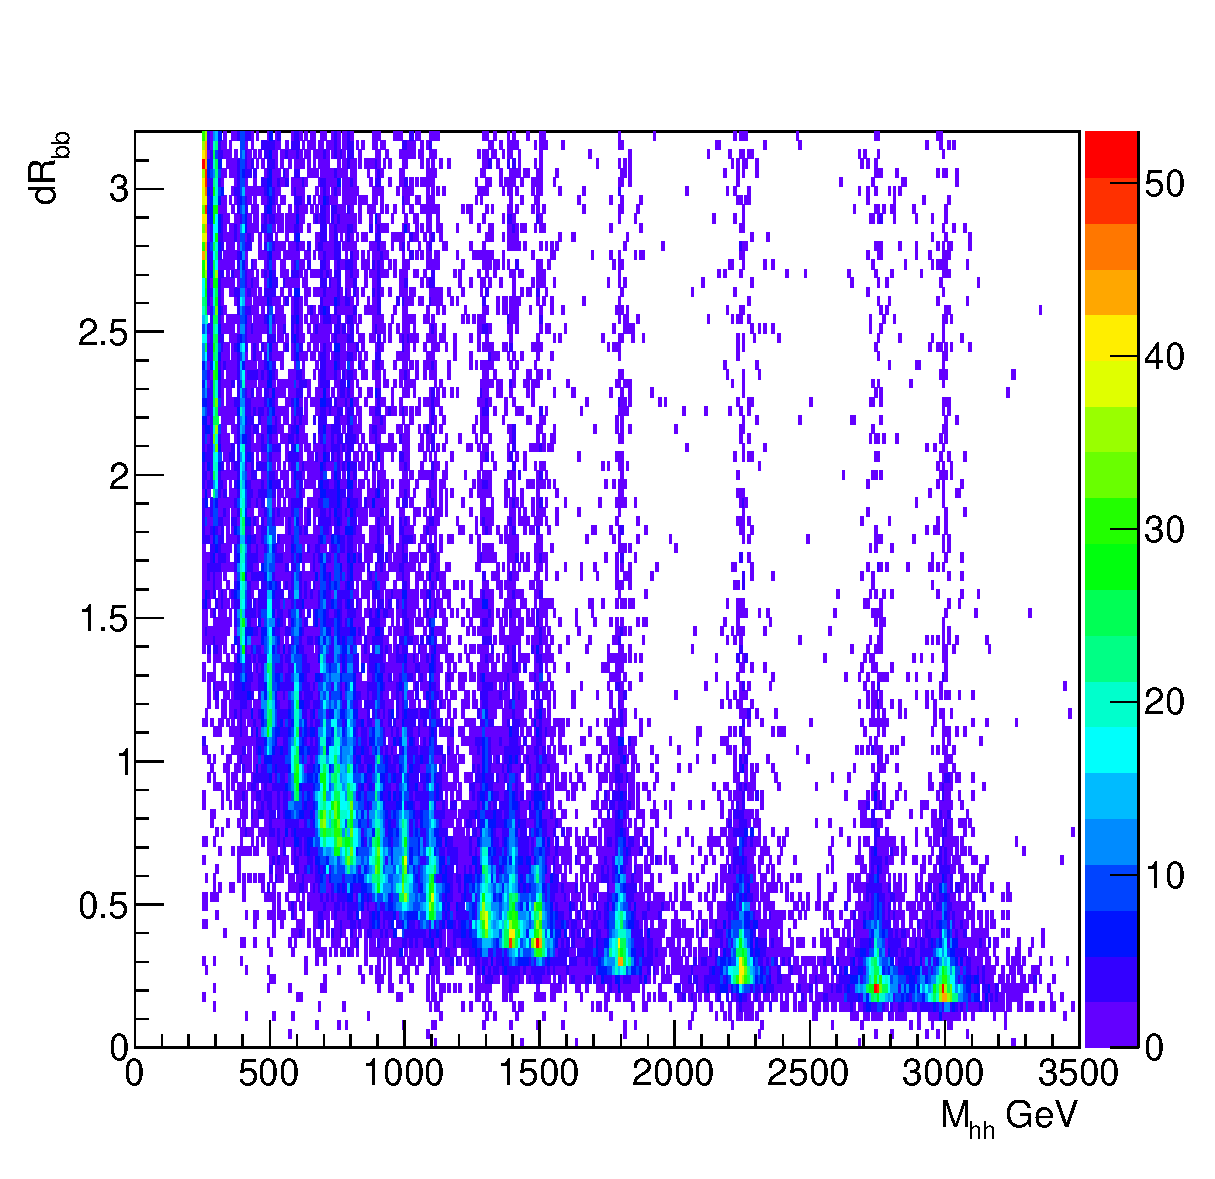
\includegraphics[scale=0.33]{DRMhhPlots_fine/drbb}
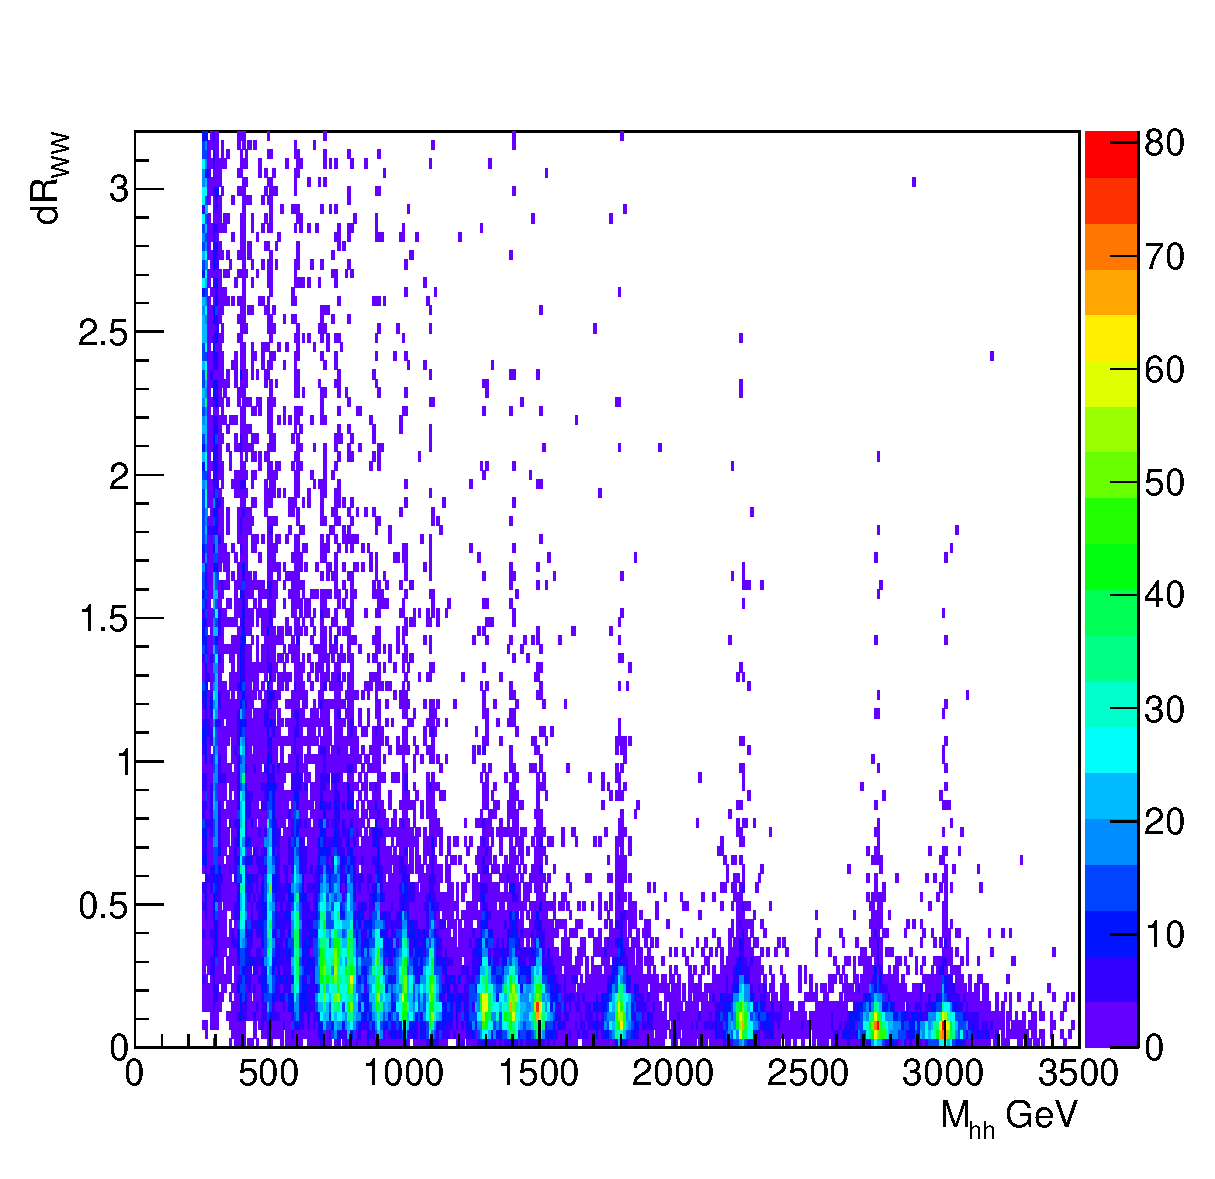
\includegraphics[scale=0.33]{DRMhhPlots_fine/drWW}
\\
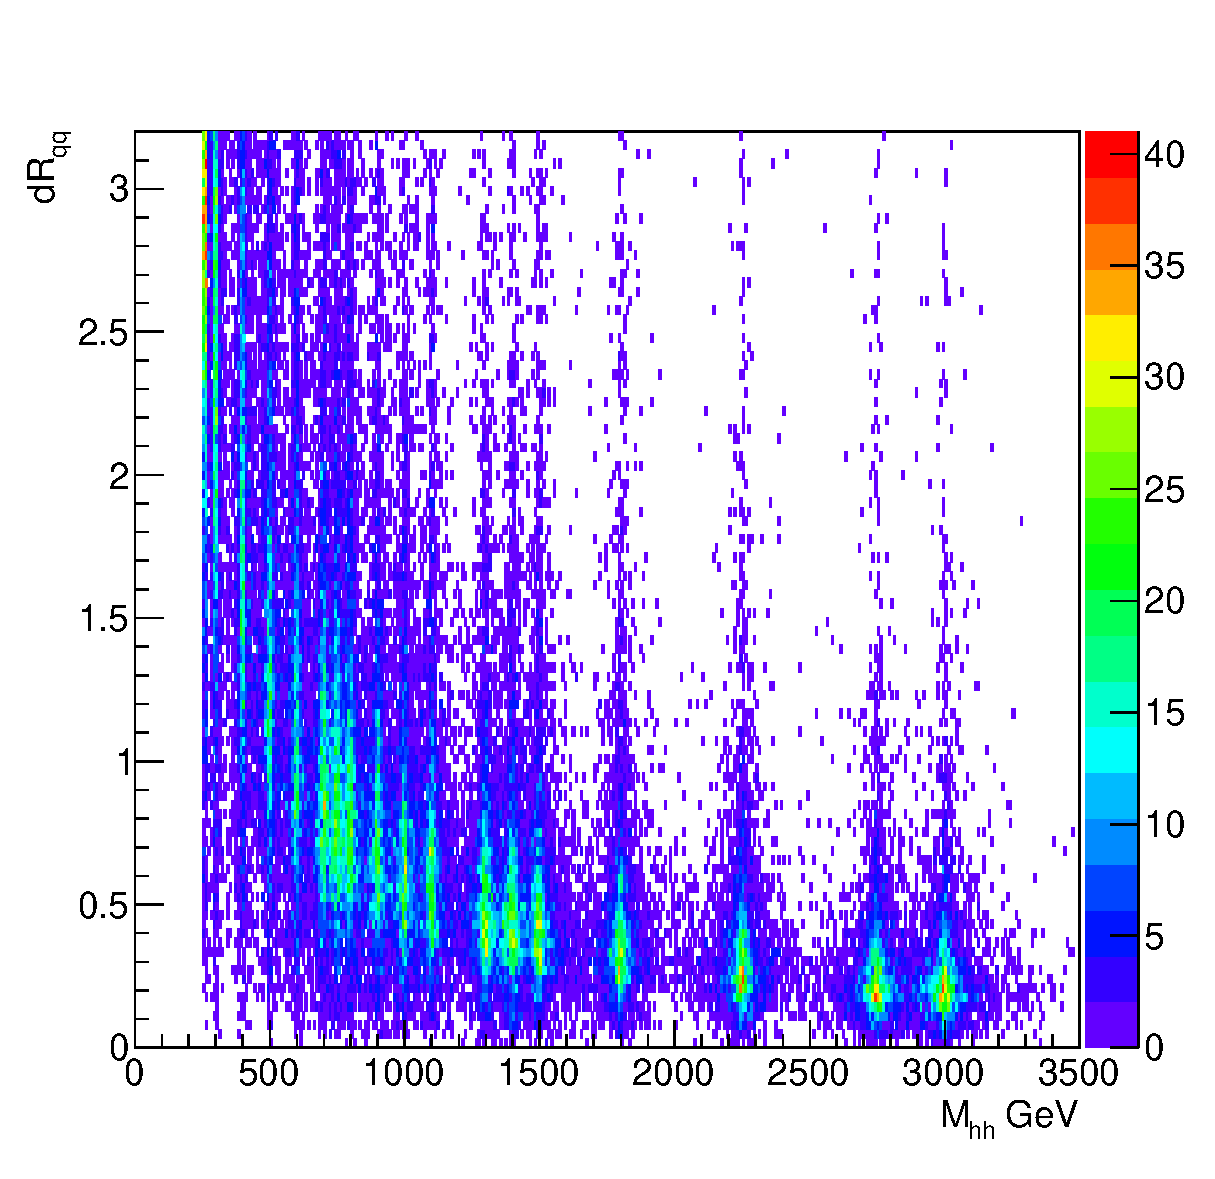
\includegraphics[scale=0.33]{DRMhhPlots_fine/drqq}
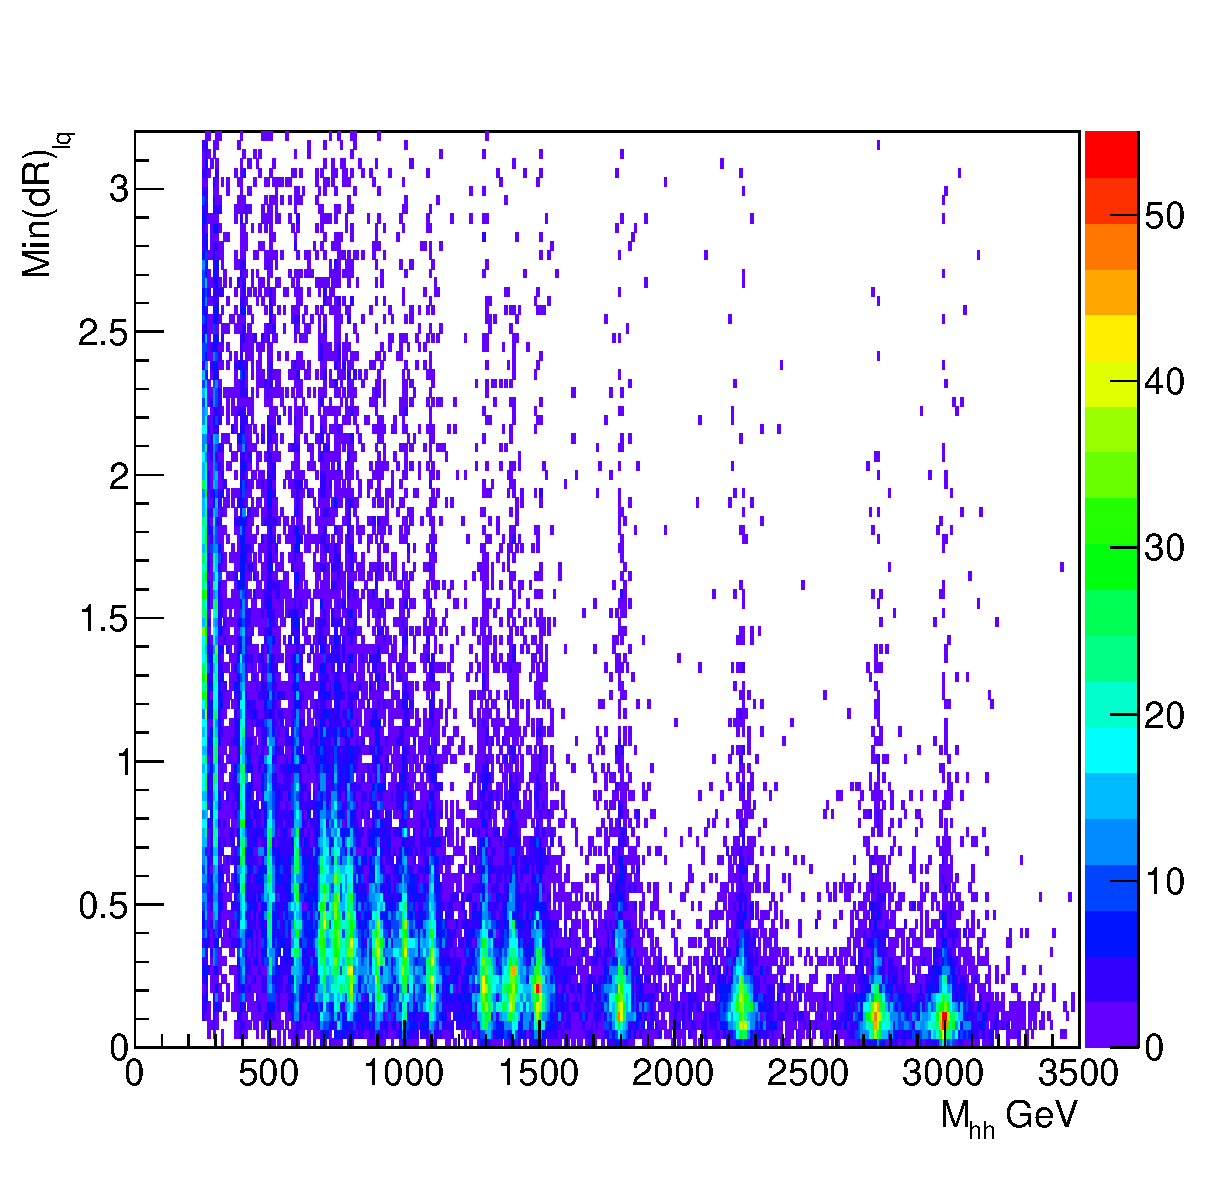
\includegraphics[scale=0.33]{DRMhhPlots_fine/drminlq}

\caption[Distance between parton objects]{Distance between the two b partons (top left); the two W bosons (top right); the two light quarks (bottom left); and the lepton and the most distant light quark (bottom right) for resonant $HH$ production as a function of resonant mass.}
\label{fig:dr}
\end{center}
\end{figure}
\indent On the ${H\rightarrow b\overline{b}}$ side, this is accounted for through the boosted analysis selection described in Secion ~\ref{sec:boosted_evtreco}. Moving toward the full Run 2 analysis, it is worthwhile to look at the potential gain from including a boosted ${H\rightarrow WW^{*}}$ selection. This ``fully-boosted" analysis can be used in conjunction with the current boosted and resolved analysis to increase sensitivity and reach.\newline
%\section{Fully Boosted Analysis}
\indent The ``fully-boosted" analysis piggybacks off of the analysis presented in Chapter ~\ref{chap:anal}. This means the data and Monte Carlo Samples , object reconstruction, and trigger requirements are the same as the previously presented analysis. \newline
\section{Event Reconstruction}
Identically to the boosted analysis, section \ref{sec:Boosted}, events are reconstructed by requiring at least one reconstructed lepton. To reconstruct the ${H\rightarrow b\overline{b}}$ candidate, there should be at least one large-R jet with ${\Delta{R} > 1.0}$ from the selected lepton. The highest of these large-R jets is selected as the ${H\rightarrow b\overline{b}}$ candidate. This large-R jet is then required to have at least two track jets associated to it. Events with a ${H\rightarrow b\overline{b}}$ in the range ${30 \text{ GeV} < m_{\mathrm{bb}} < 300 \mathrm{GeV}}$ are retained for further analysis.\newline
\indent To reconstruct the ${H\rightarrow WW^{*}}$ candidate, there should be at least one large-R jet with ${\Delta{R} < 1.0}$ from the selected lepton. This large-R jet is selected as the ${H\rightarrow WW^{*}}$ jet candidate. Once the ${H\rightarrow b\overline{b}}$ jet has been selected, they are split into either electron or muon channel for the full reconstruction.\newline
\indent Calorimeter jets are clusters of energy that are grouped together into an object based on distances. If an electron, which deposits the majority of its energy into the calorimeter, were to fall within the radius of a calorimeter jet, its energy should be measured as part of the jet energy. Using this, it is possible to use a single large-R to measure the energy of the ${W\rightarrow qq}$ system and the electron.  With the large-R jet and the \met, it is possible to fully reconstruct the ${H\rightarrow WW^{*}}$ system. The neutrino is reconstructed using a similar method as in Section ~\ref{ssec:event_reco_res}. Imposing the relation:
\begin{equation}
\label{eq:mh}
m_h^2 = (p^{\nu} + p^{\mathrm{large-R jet}})^2
\end{equation}
the neutrino $p_z$ can be reconstructed using the relations:
\[
p_E^{\nu} = E^{\nu} = \sqrt{P_T^2 + p_z^2} \quad p_x^{\nu} = P_Tcos(\phi) \quad p_y^{\nu} = P_T sin(\phi)
\]
where $\phi$ is the azimuthal angle of the $\met$, $E^{\nu}$ the neutrino energy, $p_x$ and $p_y$ the two transverse spatial components of the neutrino momentum.\newline
\indent Muons do not deposit a significant amount of energy in the calorimeters, this means we cannot use the same reconstruction as the electrons. Instead, the muons are treated in a more traditional fashion. In the muon channel, the large-R jet contains the energy of the ${W\rightarrow qq}$ system. The muon is reconstructed using the MS and ID information and the neutrino is reconstructed identically to \ref{ssec:event_reco_res}, with the hadronic $W$ as a single object.\newline
\indent Figure ~\ref{fig:topo} shows a diagram of the event topology after the event reconstruction.

\begin{figure}[h]
\begin{center}
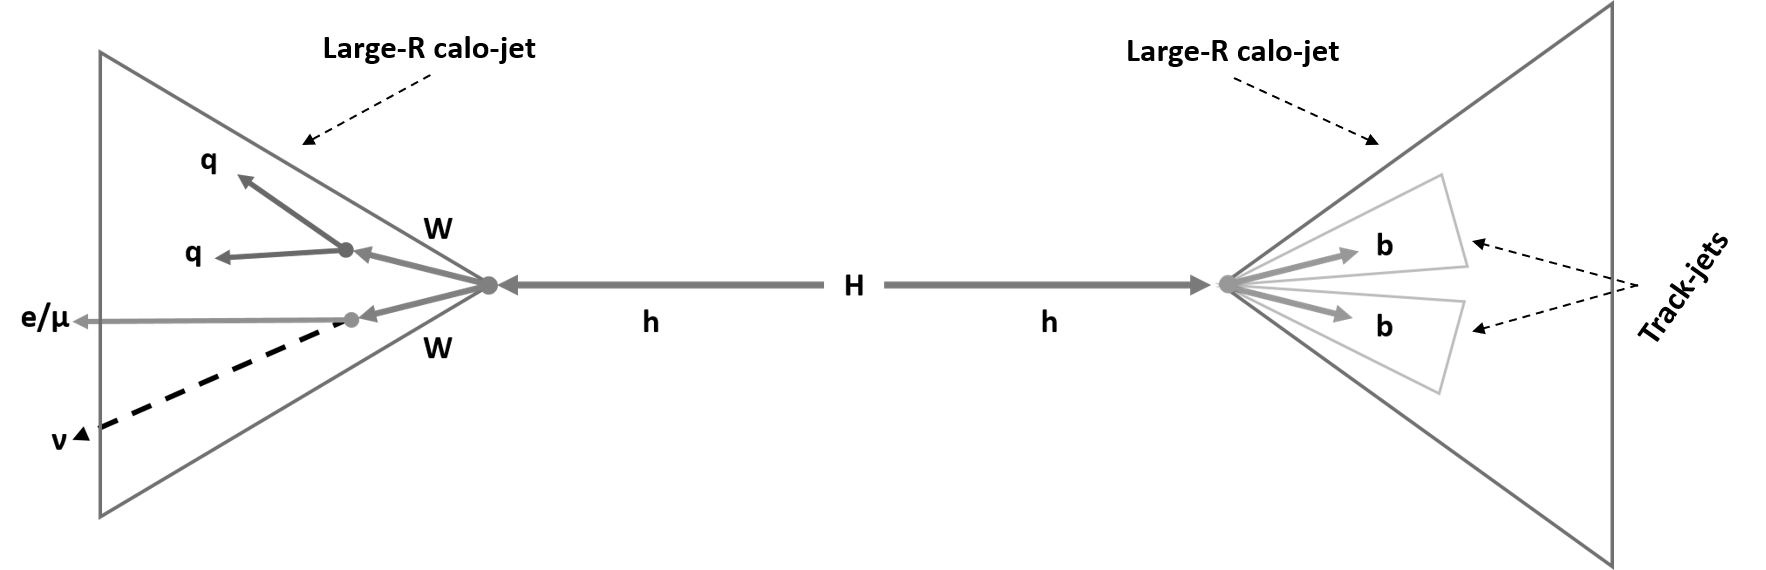
\includegraphics[scale=0.4]{figures/full_boosted}
\caption{Diagram of the fully-boosted event topology}
\label{fig:topo}
\end{center}
\end{figure}
\section{Event selection}
After the event is reconstructed, a b-tag requirement is applied to the 2 track-jets in the ${H\rightarrow b\overline{b}}$ candidate. The \met{} is required to be more than 50 GeV to reject events from QCD background. Finally a  \pt requirement is placed on the ${H\rightarrow WW^{*}}$ candidate. It is important to cut on the same physics objects. To accomplish this, an ``adjusted \pt" (${\pt^{'}}$) cut of 250 GeV is applied. Table ~\ref{tab:adjpt} defines the ${\pt^{'}}$ for both channels. 


\begin{table}
\begin{center}
\begin{tabular}{l|c}
\hline
\\
Lepton Channel & Alternative \pt definition \\
\hline
Muon Channel & ${\pt^{'} = \pt^{\mathrm{Large-R jet}}}$\\
\hline
\\
Electron channel & ${\pt^{'} = \sqrt{(p_{x}^{\mathrm{Large-R jet}} - p_{x}^{\mathrm{electron}})^{2}+(p_{y}^{\mathrm{Large-R jet}} - p_{y}^{\mathrm{electron}})^{2}}}$
\end{tabular}
\caption[Alternative \pt definition for the electron and muon channels]{Alternative \pt definition for the electron and muon channels. A cut of $\pt^{'} > 250 \text{ GeV}$ is applied to the selected ${H\rightarrow WW^{*}}$ large-R jet.}
\label{tab:adjpt}
\end{center}
\end{table}

\subsection{Comparison of reconstruction objects}
Figure \ref{fig:elec_sel} and \ref{fig:muon_sel} show a comparison of the old boosted analysis reconstruction and the new fully-boosted analysis for the electron and muon selection respectively. The $m_{WW^*{}}$ distribution shows a much shorter tail in the fully-boosted analysis than in the old boosted analysis. Along with this, the $m_{HH}$ distribution has a sharper peak around the resonant mass. A sharper peak allows for tighter cuts around the signal mass, leading to a better signal/background ratio.



\begin{figure}[h]
\begin{center}
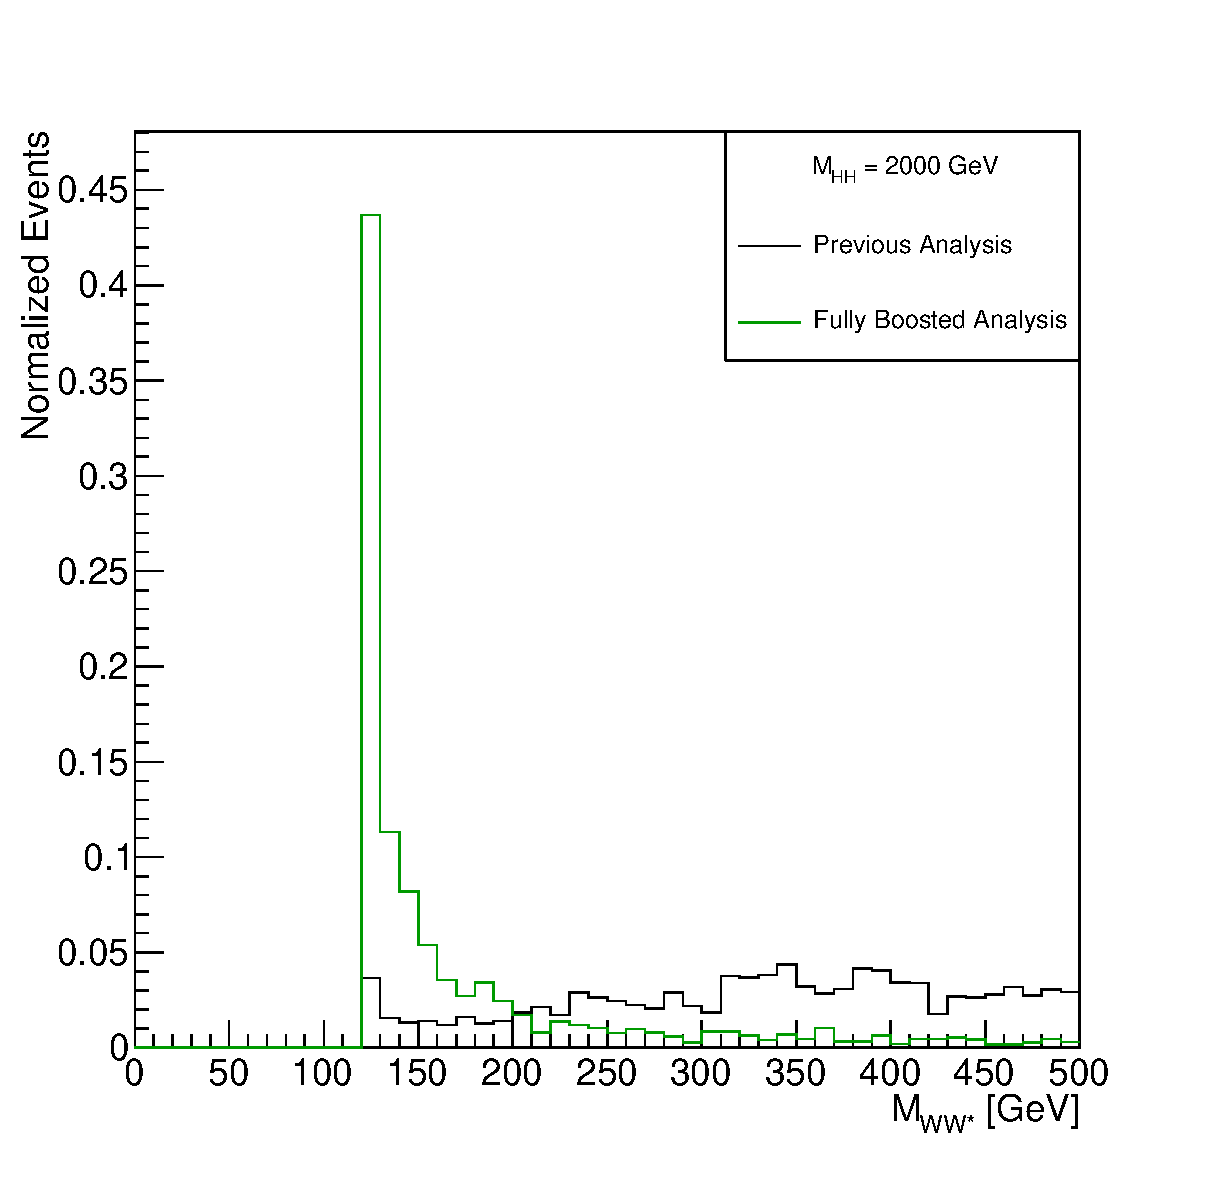
\includegraphics[scale=0.25]{figures/WHad_plots_john_withcuts/electron/hww_m_Xhh2000}
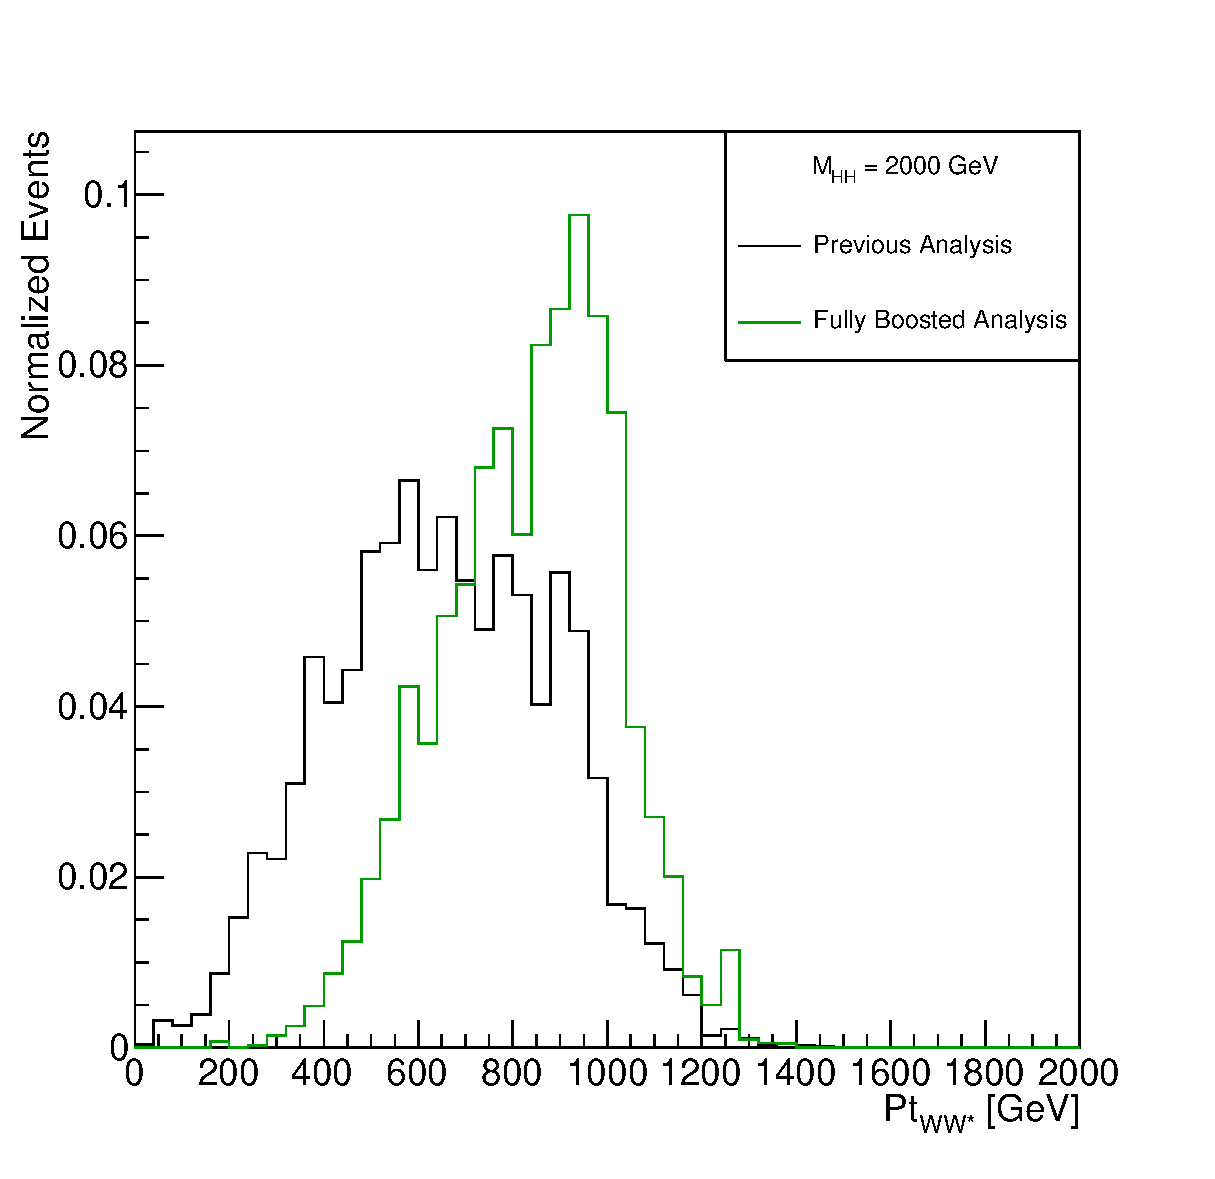
\includegraphics[scale=0.25]{figures/WHad_plots_john_withcuts/electron/hww_pt_Xhh2000}\\
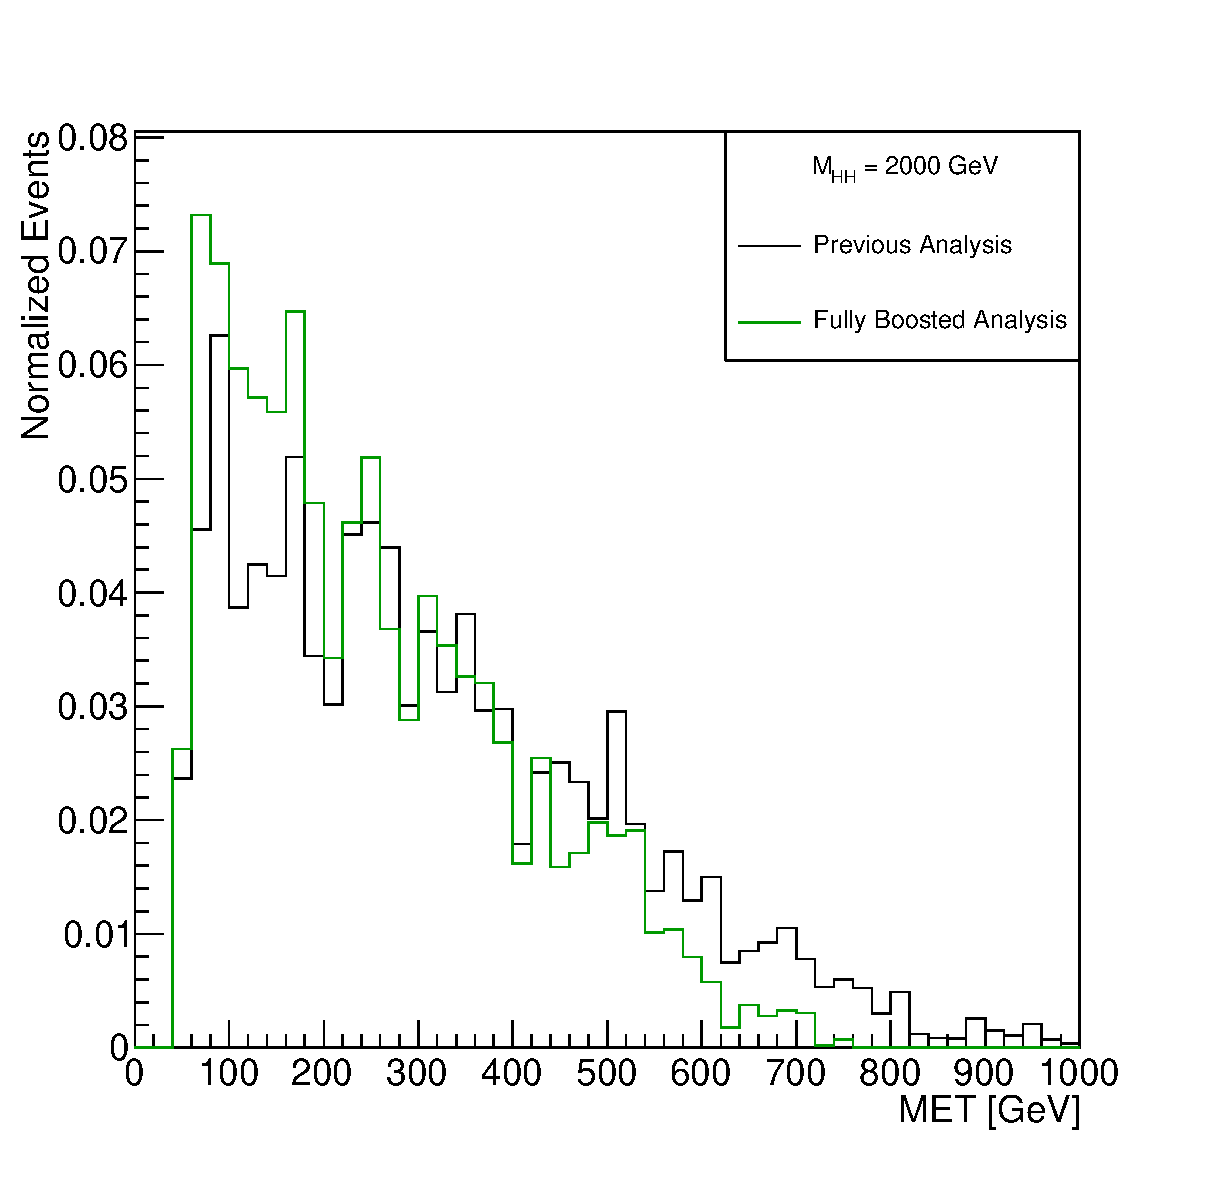
\includegraphics[scale=0.25]{figures/WHad_plots_john_withcuts/electron/wlep_met_Xhh2000}
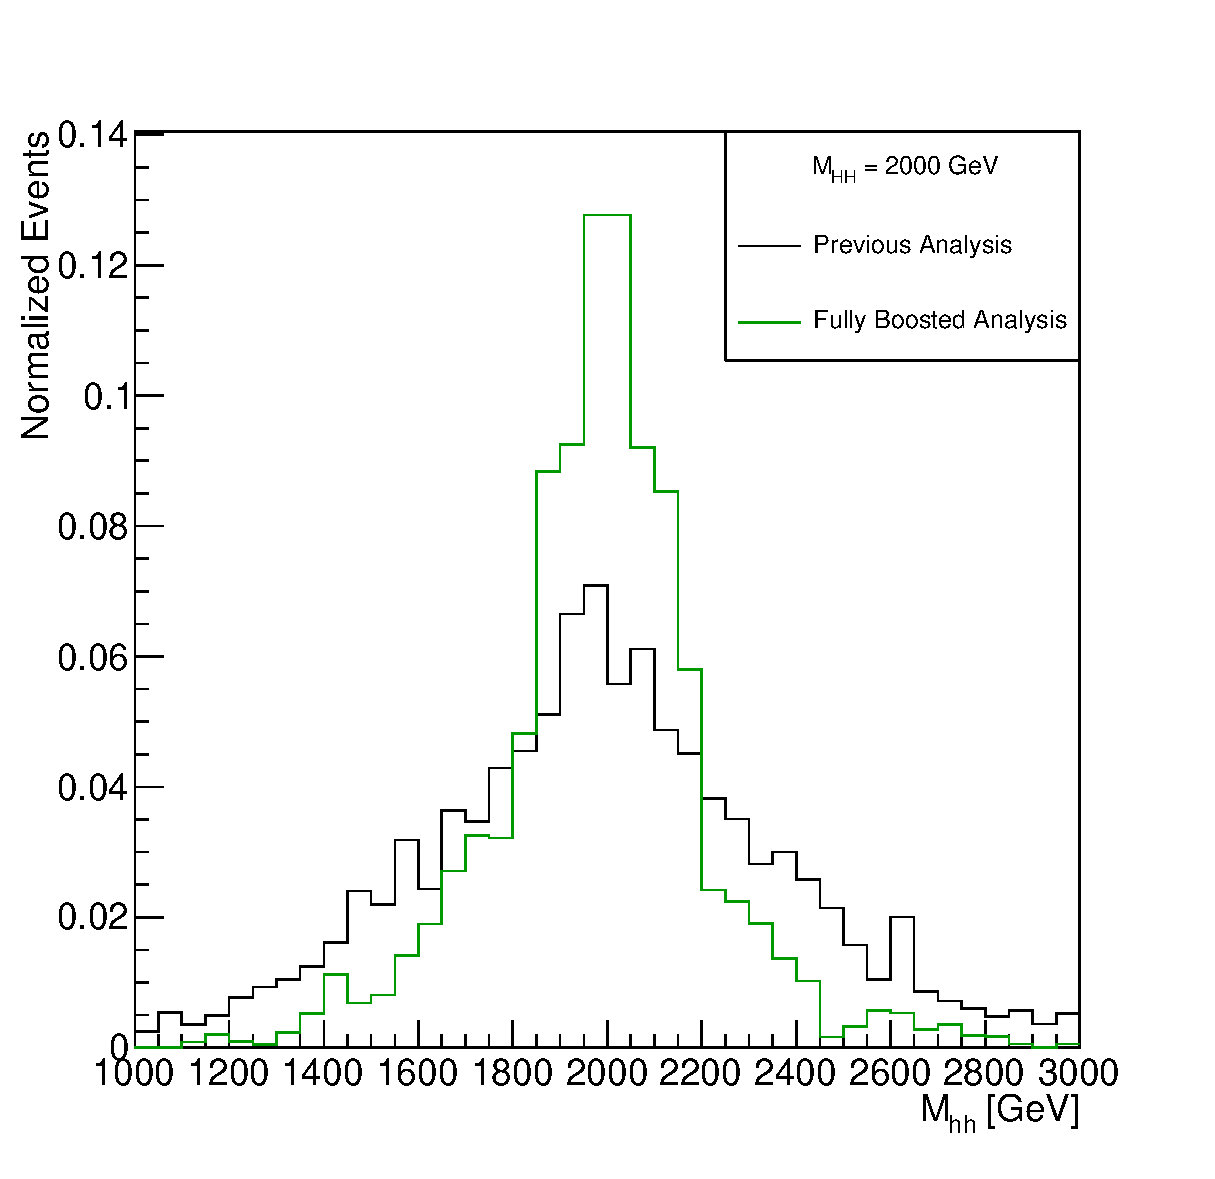
\includegraphics[scale=0.25]{figures/WHad_plots_john_withcuts/electron/hh_m_Xhh2000}
\caption[Comparison of ${H\rightarrow WW^{*}}$ mass, ${H\rightarrow WW^{*}}$ \pt, \met , and $HH$ mass for the electron channel]{Comparison of reconstructed ${H\rightarrow WW^{*}}$ mass (top left), ${H\rightarrow WW^{*}}$ \pt (top right), \met (bottom left), and $HH$ mass for the  previous boosted analysis reconstruction and new fully boosted selection for a resonant signal with a mass of 2000 GeV in the electron channel.}
\label{fig:elec_sel}
\end{center}
\end{figure}

\newpage

\begin{figure}[h]
\begin{center}
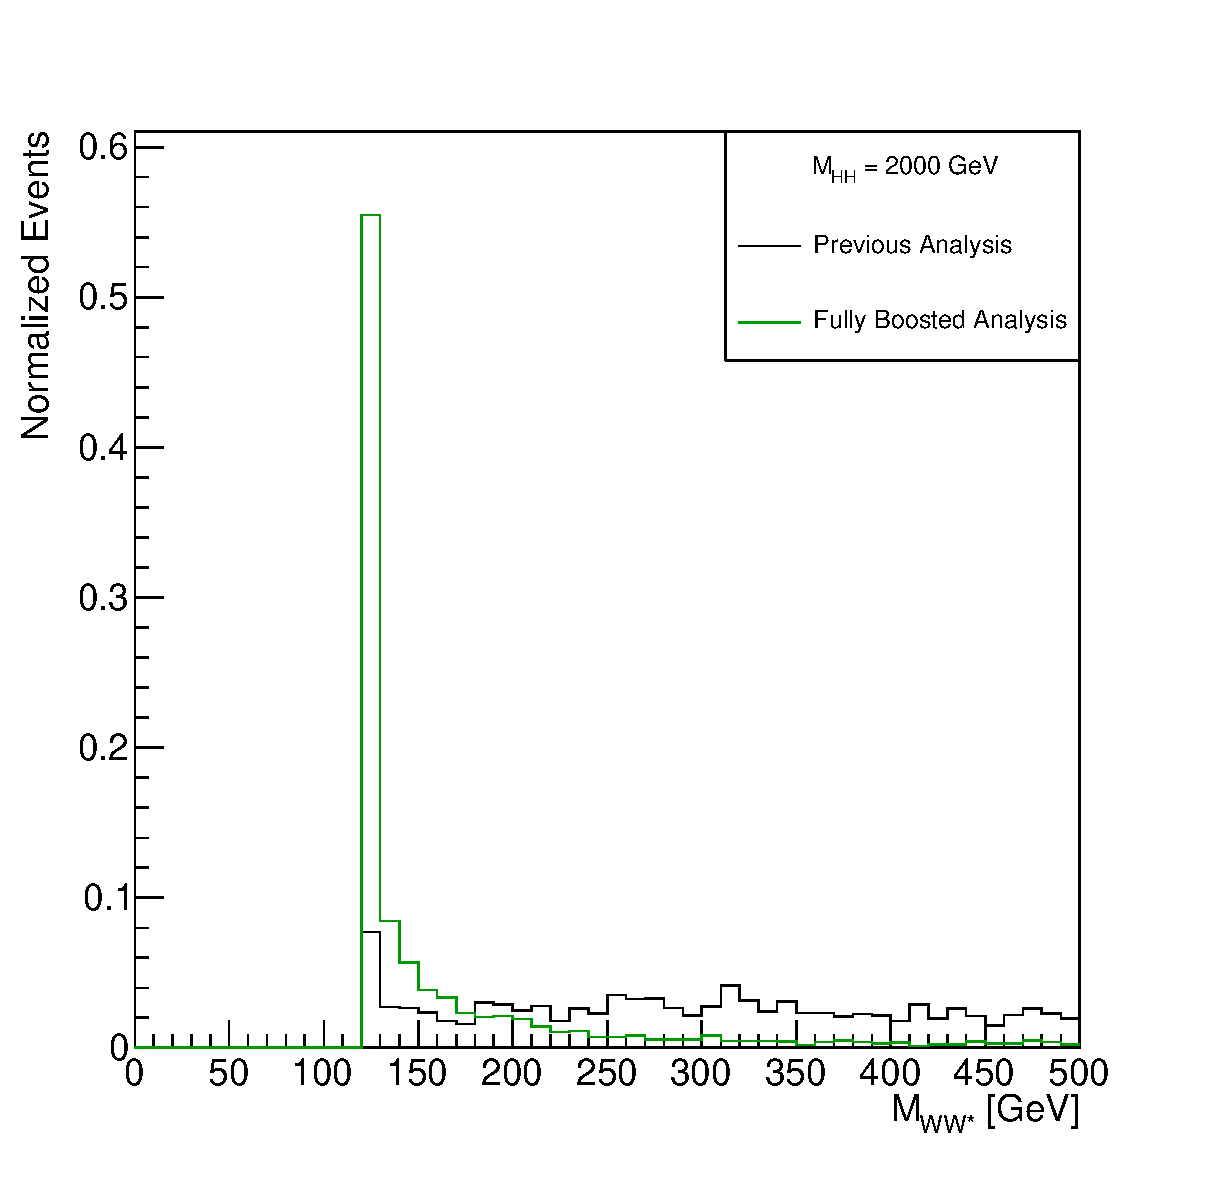
\includegraphics[scale=0.25]{figures/WHad_plots_john_withcuts/muon/hww_m_Xhh2000}
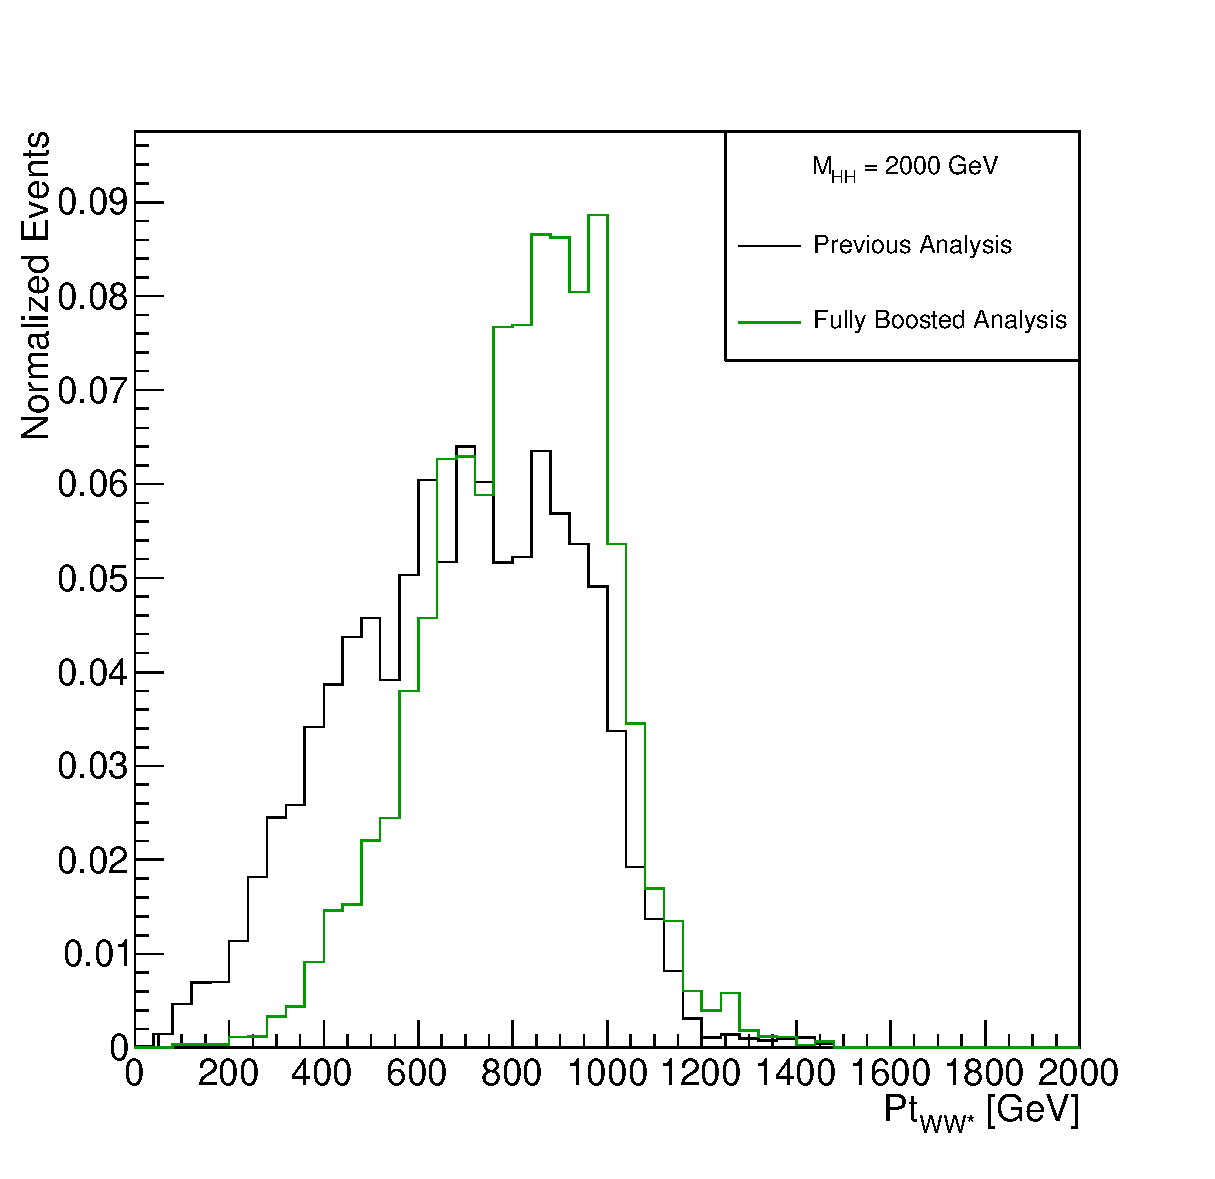
\includegraphics[scale=0.25]{figures/WHad_plots_john_withcuts/muon/hww_pt_Xhh2000}\\
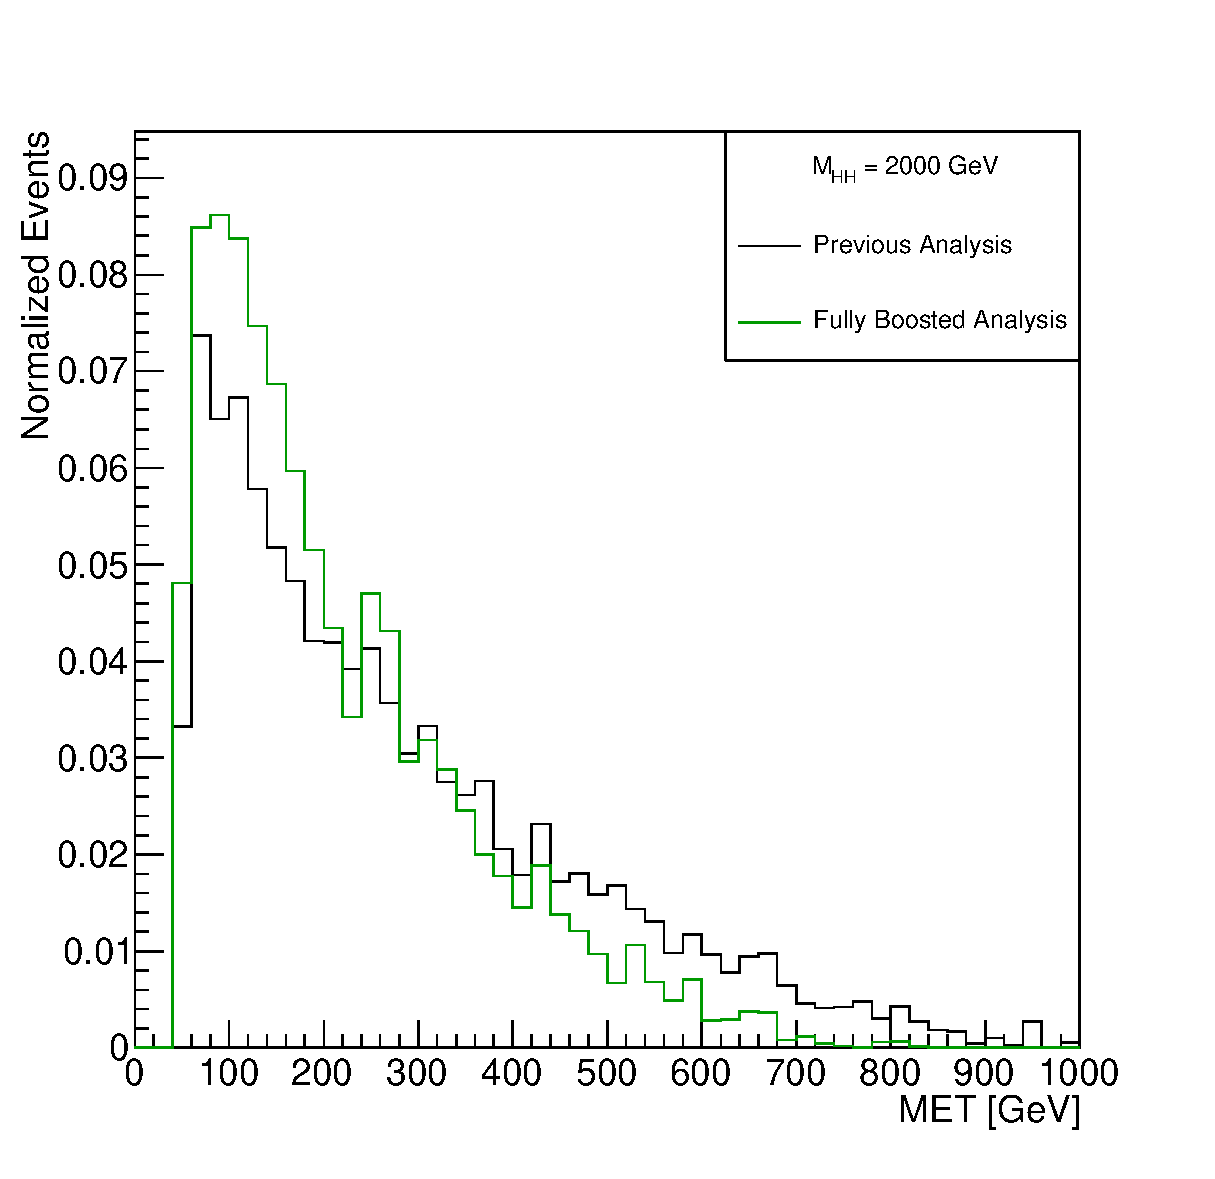
\includegraphics[scale=0.25]{figures/WHad_plots_john_withcuts/muon/wlep_met_Xhh2000}
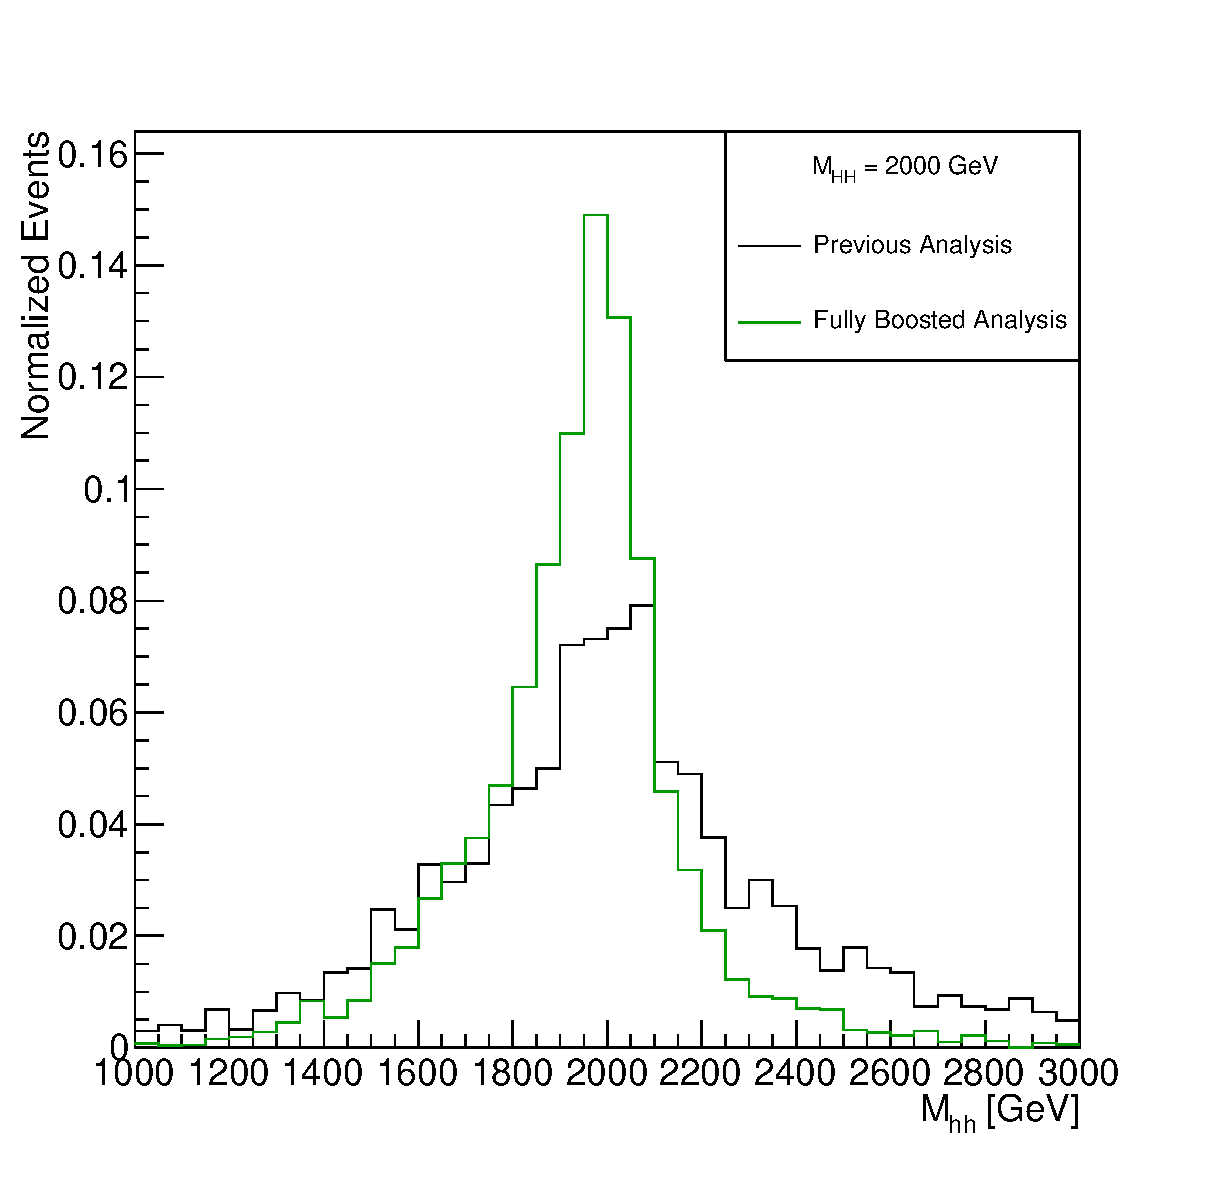
\includegraphics[scale=0.25]{figures/WHad_plots_john_withcuts/muon/hh_m_Xhh2000}
\caption[Comparison of ${H\rightarrow WW^{*}}$ mass, ${H\rightarrow WW^{*}}$ \pt, \met , and $HH$ mass for the muon channel]{Comparison of ${H\rightarrow WW^{*}}$ mass (top left), ${H\rightarrow WW^{*}}$ \pt (top right), \met (bottom left), and $HH$ mass for the  previous boosted analysis reconstruction and new fully boosted selection for a resonant signal with a mass of 2000 GeV in the muon channel.}
\label{fig:muon_sel}
\end{center}
\end{figure}





\subsection{Signal Region Definition}
As with the boosted analysis in Section ~\ref{sec:Boosted}, the ${h\rightarrow b\overline{b}}$ candidate must have a jet mass in the window ${90 \text{ GeV } < m_{bb} < 140 \text{ GeV}}$ to be considered in the signal region (SR). The previous boosted analysis included a b-jet veto for all jets outside of the ${H\rightarrow b\overline{b}}$ candidate. In order to increase statistics for the QCD multijet estimate, this requirement was removed from the fully boosted analysis.

\subsection{mBB Control Region}
To check the modeling of the background, a control region is created with an inverted ${m_{bb}}$ cut. Section ~\ref{ssec:mbbcr_plots_whad} shows various kinematic distributions in  the mBB control region to check the background shape with respect to data.
\subsection{Multijet Background}
The QCD multijet background is estimated using the same data-driven background as the boosted analysis. The ABCD method with the regions defined as:
\begin{itemize}
\item Region A: \met $>$ 50 GeV, $|d_{0}^{\textrm{sig}}|$ $<$ 2.0
\item Region B: \met $<$ 50 GeV, $|d_{0}^{\textrm{sig}}|$ $<$ 2.0
\item Region C: \met $>$ 50 GeV, $|d_{0}^{\textrm{sig}}|$ $>$ 2.0
\item Region D: \met $<$ 50 GeV, $|d_{0}^{\textrm{sig}}|$ $>$ 2.0
\end{itemize}

\subsubsection{Yield Prediction}
Table \ref{tab:boosted_region_bd_promptbkgd_data_new} lists the MC predicted prompt lepton backgrounds, observed data and calculated multijet yields in Region B and D before the ${H\rightarrow b\overline{b}}$ mass cut is applied and Table \ref{tab:boosted_region_c_promptbkgd_data_new} shows the yields in Region C mBB control region and signal region.\newline

\begin{table}
\begin{center}
\begin{tabular}{l|c|c||c|c}
             &\multicolumn{2}{c||}{Region B}                &\multicolumn{2}{c}{Region D} \\
\hline
Samples       & Electron               & Muon                & Electron          & Muon \\      
\hline
$t\bar{t}$    &  138.7 $\pm$ 7.3      & 146.1 $\pm$ 8.3      & 14.4 $\pm$ 2.7    & 6.3  $\pm$ 1.5  \\
W+Jets        &  27.3 $\pm$ 1.7       & 27.9 $\pm$ 1.9       & 1.1 $\pm$ 0.3    & 2.0  $\pm$ 0.4  \\        
Single-top    &  7.1  $\pm$ 1.4       & 5.2  $\pm$ 1.4     &  0.2 $\pm$ 0.2    &  0.4  $\pm$ 0.3  \\
Z+Jets        &  18.3  $\pm$ 0.8       & 9.3  $\pm$ 0.5     &  1.9 $\pm$ 0.3    &  0.9  $\pm$ 0.2  \\
Dibosons      &  3.1  $\pm$ 0.5       & 1.3  $\pm$ 0.3     &  0.2 $\pm$ 0.1    &  0.2  $\pm$ 0.1  \\
\hline
Total Prompt  &  194.4 $\pm$ 7.7      & 189.9 $\pm$ 8.7    & 17.8 $\pm$ 2.7    & 9.8  $\pm$ 1.6  \\
\hline
Data          &  274.0  $\pm$ 16.6      & 218.0   $\pm$ 14.8    & 34.0  $\pm$ 5.8   & 30.0   $\pm$ 5.5  \\
\hline
QCD           & 79.6 $\pm$ 18.3       & 28.1 $\pm$ 17.1    & 16.2 $\pm$ 6.4  & 20.2 $\pm$ 5.7 \\
\end{tabular}
\end{center}
\caption[MC predicted prompt lepton backgrounds, observed data and calculated multijet yields
in Region B and D]{MC predicted prompt lepton backgrounds, observed data and calculated multijet yields
in Region B and D. The multijet yield is calculated by subtracting the estimated total prompt lepton
backgrounds from the observed data. The statistical uncertainty on the yields is shown.}
\label{tab:boosted_region_bd_promptbkgd_data_new}
\end{table}


\begin{table}
\begin{center}
\begin{tabular}{l|c|c||c|c}
             &\multicolumn{2}{c||}{mBBcr}               &\multicolumn{2}{c}{SR}\\
\hline
Samples       & Electron            & Muon               & Electron         & Muon     \\      
\hline
$t\bar{t}$          &   21.7	$\pm$ 4.1   &   12.8 $\pm$ 2.1	&  	6.4 $\pm$ 1.4		& 	5.4 $\pm$ 1.2\\
W+Jets          &   3.4 	$\pm$ 0.6   &    2.3 $\pm$ 0.3	&	1.4 $\pm$ 0.3		&  	1.2 $\pm$ 0.3\\
Single-top      &   0.7 	$\pm$ 0.5   &    0.3 $\pm$ 0.2	&	0.4 $\pm$ 0.3       	&  	0.2 $\pm$ 0.2\\
Z+Jets          &   1.0 	$\pm$ 0.2   &    0.4 $\pm$ 0.1	& 	0.4 $\pm$ 0.1        & 	0.2 $\pm$ 0.1\\
Dibosons   &   0.2 	$\pm$ 0.1   &    0.0 $\pm$ 0.0	&	0.1 $\pm$ 0.1       	& 	0.0 $\pm$ 0.0\\
\hline
Total Prompt         &   26.9 	$\pm$ 4.1   &   15.9 $\pm$ 2.2	&	8.7 $\pm$ 1.5       	& 	7.0 $\pm$ 1.3\\
\hline
Data           &   53.0 $\pm$ 7.3   &   33.0 $\pm$ 5.7	&	12.0 $\pm$ 3.5      	& 	20.0 $\pm$ 4.5\\
\hline
QCD            &   26.1 $\pm$ 8.4   &   17.1 $\pm$ 6.1	&	3.3 $\pm$ 3.8       	& 	13.0 $\pm$ 4.7\\
\end{tabular}
\end{center}
\caption[MC predicted prompt lepton backgrounds, observed data and calculated multijet yields
in Region C mBBcr and SR]{MC predicted prompt lepton backgrounds, observed data and calculated multijet yields
in Region C mBBcr and SR. The multijet yield is calculated by subtracting the estimated total prompt lepton
backgrounds from the observed data. The statistical uncertainty on the yields is shown.}
\label{tab:boosted_region_c_promptbkgd_data_new}
\end{table}


\indent Table \ref{tab:boosted_bkgd_abcd_ratio_new} shows the ratio in the electron channel and muon channel.
The predicted yields of the QCD multijet background in the mBB control region and signal region are presented in table \ref{tab:boosted_bkgd_abcd_yield_new}. The QCD multijet background is estimated to be 13\% of the total background in the signal region (Table \ref{tab:boosted_bkgd_mbbcr_yields_new}).

\begin{table}
\begin{center}
\begin{tabular}{c|c|c}
Multijet yield in region              & Electron                & Muon   \\      
\hline
$N_B^\text{QCD}$                      & 79.6 $\pm$ 18.3      & 28.1 $\pm$ 17.1 \\
$N_D^\text{QCD}$                      & 16.2 $\pm$ 6.4      & 20.2 $\pm$ 5.7  \\
\hline
$N_{B}^\text{QCD}$/$N_{D}^\text{QCD}$     & 4.9 $\pm$ 2.62 (46.0\%) & 1.4 $\pm$ 0.94 (67.2\%)   \\
\end{tabular}
\end{center}
\caption[Multijet yields in region B and region D and also the ratio of the yields for each lepton channel]{Multijet yields in region B and region D and also the ratio of the yields for each lepton channel. The error
on the $\frac{N_B^\text{QCD}}{N_D^\text{QCD}}$ ratio is propagated from the statistical uncertainties on the multijet yields in each region.}
\label{tab:boosted_bkgd_abcd_ratio_new}
\end{table}

\begin{table}[!htbp]
\begin{center}
\begin{tabular}{c|c|c}
Multijet yield in region & Electron  & Muon  \\  
\hline
\multicolumn{3}{c}{SR} \\
\hline
$N_C^\text{QCD}$         & 3.3  $\pm$ 3.8 & 13.0 $\pm$ 4.7 \\
$N_A^\text{QCD}$         & 16.4 $\pm$ 20.5 (126.8\%) & 18.1 $\pm$ 13.9 (76.8\%) \\
\hline
\multicolumn{3}{c}{mBBcr} \\
\hline
$N_C^\text{QCD}$       & 26.1  $\pm$ 8.4 & 17.1  $\pm$ 6.1  \\
$N_A^\text{QCD}$       & 128.3 $\pm$ 79.4 (61.9\%) & 23.9 $\pm$ 18.1 (75.7\%)  \\
\hline
\end{tabular}
\end{center}
\caption[Multijet yield in region C and predicted yield in region A in the SR]{Multijet yield in region C and predicted yield in region A in the SR. The error on $N_A^\text{QCD}$
are propagated from the error on the $N_B^\text{QCD}$/$N_D^\text{QCD}$ ratio and statistical uncertainty on $N_C^\text{QCD}$ yield.
The numbers in brackets are the relative uncertainty in percentage.}
\label{tab:boosted_bkgd_abcd_yield_new}
\end{table}


\subsubsection{Shape prediction}
See Section \ref{sec:boosted_bkgd_qcdmultijet_shape}.

\subsubsection{Multijet yield uncertainties}
\label{sec:boosted_bkgd_qcdmultijet_yield_unc}
 
%%%%%%%%%%%%%%%%%%%%%%%%%%%%%%%
% Statistical
%%%%%%%%%%%%%%%%%%%%%%%%%%%%%%%
\paragraph{Statistical} 
The uncertainty on the predicted yield of the multijet background is determined by propagating the statistical uncertainty
of the $\frac{N_B^\text{QCD}}{N_D^\text{QCD}}$ ratio, as shown in Table~\ref{tab:boosted_bkgd_abcd_ratio_new}, and the statisical
uncertainty on the multijet yield in region C ($N_C^\text{QCD}$), as in Table~\ref{tab:boosted_bkgd_abcd_yield_new}.
 
\paragraph{1-tag/2-tag jet mass acceptance} 
Another source of uncertainty on the multijet yield is the  
the difference of acceptance of the large-$R$ jet mass cut between the single b-tag (1-tag) and two b-tag (2-tag) selections.
This uncertainty is included since the template for or the multijet shape prediction uses the multijet shape
from the 1-tag region C. Table~\ref{tab:boosted_syst_qcd_norm_mBBAcc} shows the acceptance
of the large-$R$ jet mass signal and mBB control region selection in the multijet 1-tag region C and 2-tag region C yields.
The relative difference between the acceptance in 1-tag region C and in 2-tag region C is considered as an uncertainty on the normalization
of the QCD multijet prediction.
 
\begin{table}[!htbp]
\begin{center}
\begin{tabular}{c|c|c}
\hline
Region    & Electron          & Muon      \\
\hline
\multicolumn{3}{c}{SR} \\
\hline
1-tag $\frac{N_\text{SR}}{N_\text{Inc}}$ &  32\% & 23 \% \\
2-tag $\frac{N_\text{SR}}{N_\text{Inc}}$ &  11\% & 43 \% \\
\hline \hline
Rel. difference between 1-tag and 2-tag & 26.4 \% & 46 \% \\
\hline
\multicolumn{3}{c}{mBBcr} \\
\hline
1-tag $\frac{N_\text{mBBcr}}{N_\text{Inc}}$ &  68\% & 77 \% \\
2-tag $\frac{N_\text{mBBcr}}{N_\text{Inc}}$ &  89\% & 56 \% \\
\hline \hline
Rel. difference between 1-tag and 2-tag &  24 \% &   37 \% \\
\end{tabular}
\end{center}
\caption[The acceptance of the large-$R$ jet mass signal region selection on the multijet
1-tag and 2-tag region C]{The acceptance of the large-$R$ jet mass signal region selection on the multijet
1-tag and 2-tag region C. $N_\text{SR}$($N_\text{Inc}$) is the multijet yield
with (without) the signal region large-$R$ jet mass selection.}
\label{tab:boosted_syst_qcd_norm_mBBAcc}
\end{table}
 
\subsection{mBBcr Plots}
\label{ssec:mbbcr_plots_whad}
Figure ~\ref{fig:mbbcr_plots} shows the $m_{HH}$ distribution in the mbb control region for the electron and muon channels. The figure shows a reasonable agreement between data and background in the mBB control region but with large uncertainties. Appendix ~\ref{app:fully_mbb_plots} has a more complete set of kinematic plots. 

\newpage
\begin{figure}[H]
\begin{center}
%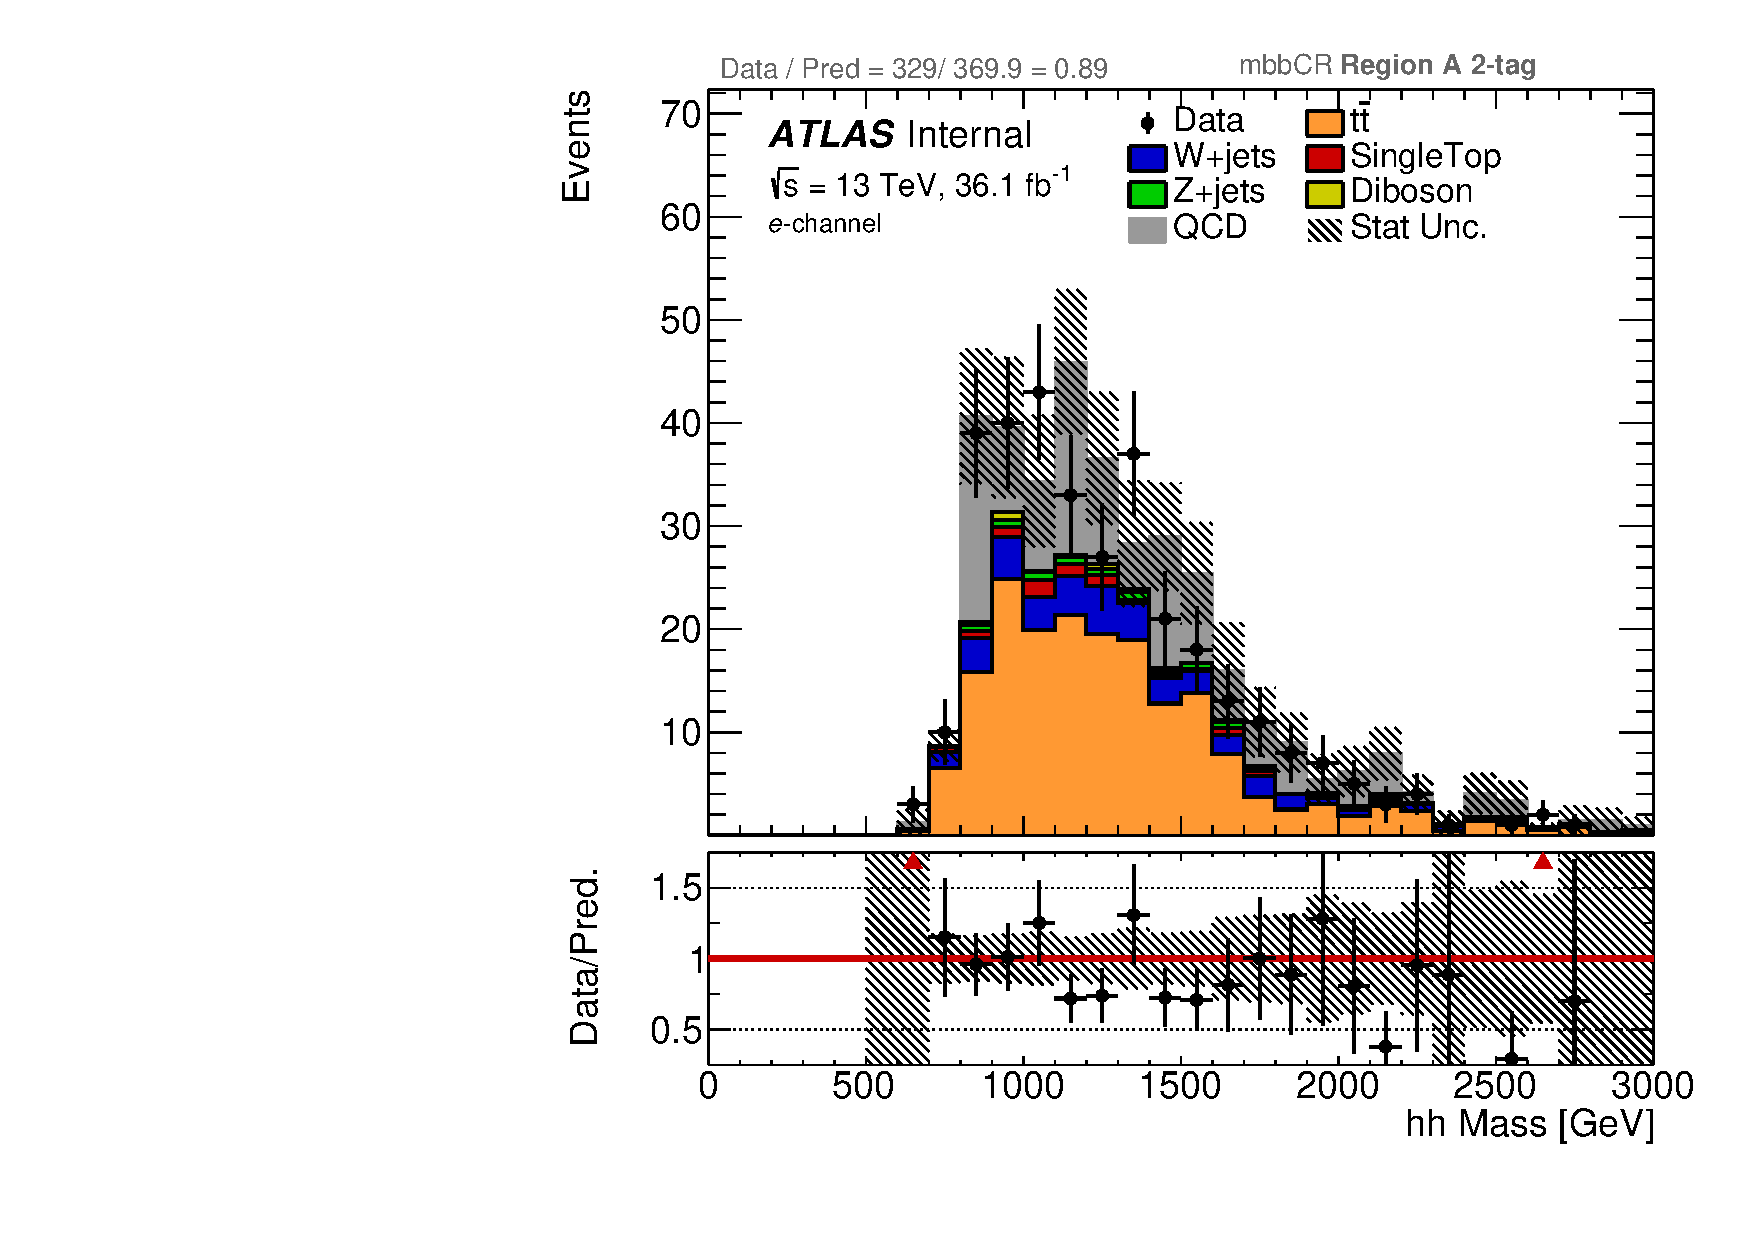
\includegraphics[scale=0.33]{figures/abcd_plots/elec_mbbcr_RegionA_hhMass_withDD}
%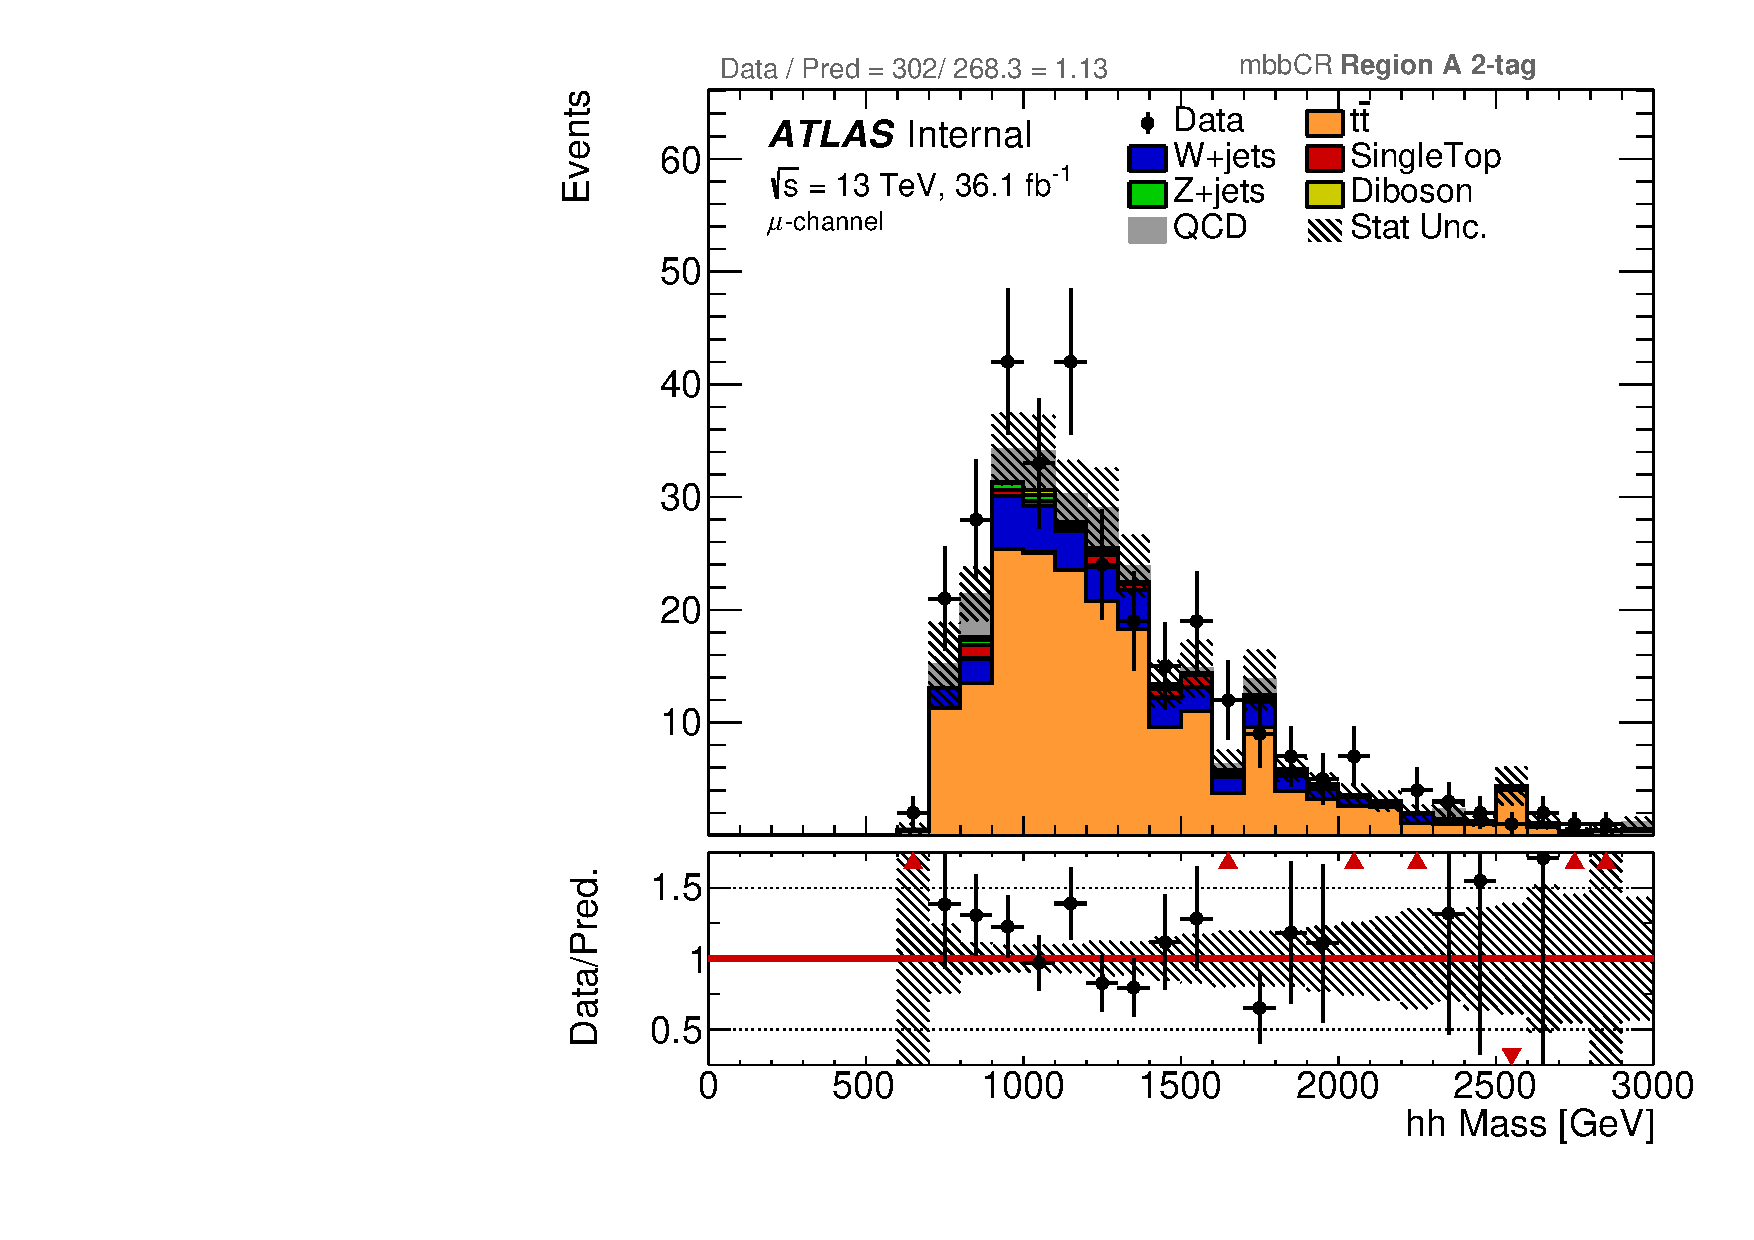
\includegraphics[scale=0.33]{figures/abcd_plots/muon_mbbcr_RegionA_hhMass_withDD}\\
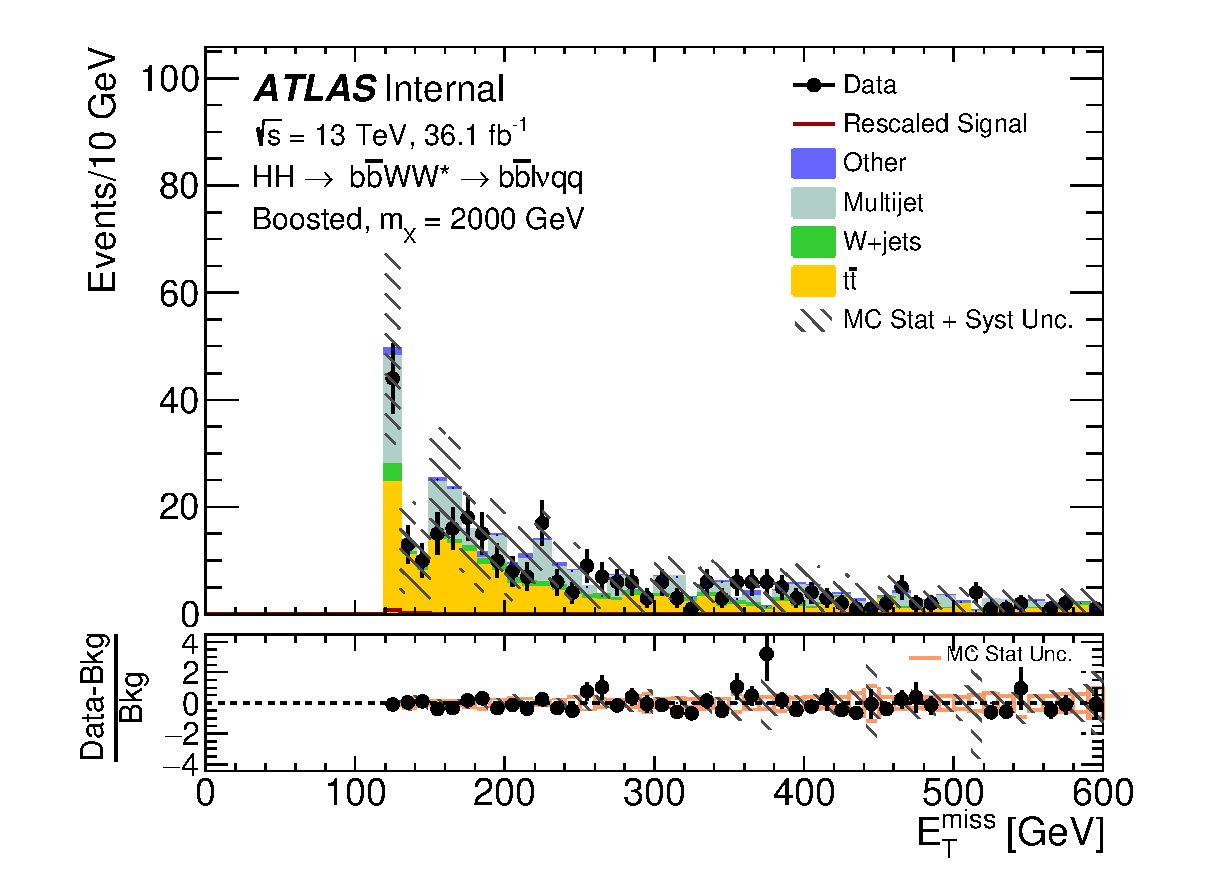
\includegraphics[scale=0.33]{figures/kinplots/C_2tag_mbbcr_elec_presel_met50_WWMass}
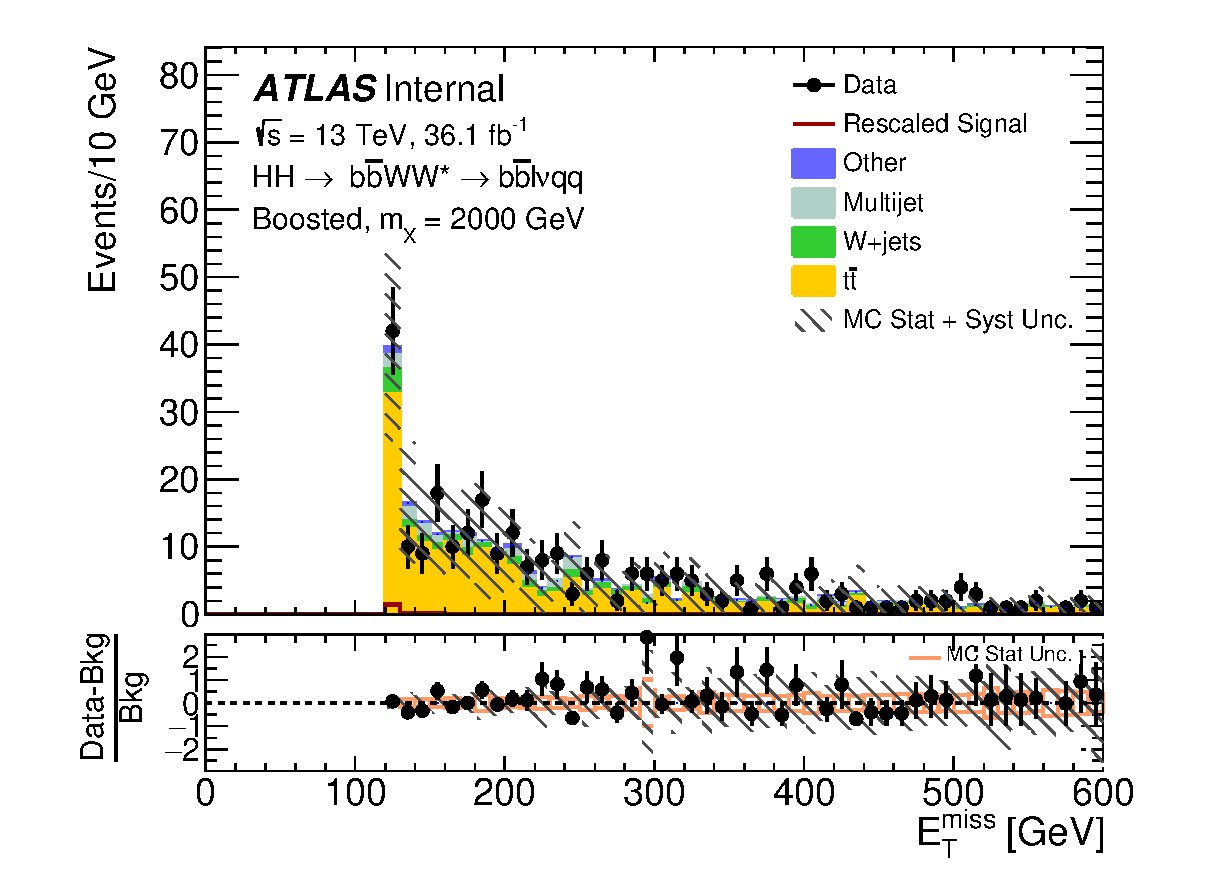
\includegraphics[scale=0.33]{figures/kinplots/C_2tag_mbbcr_muon_presel_met50_WWMass}\\
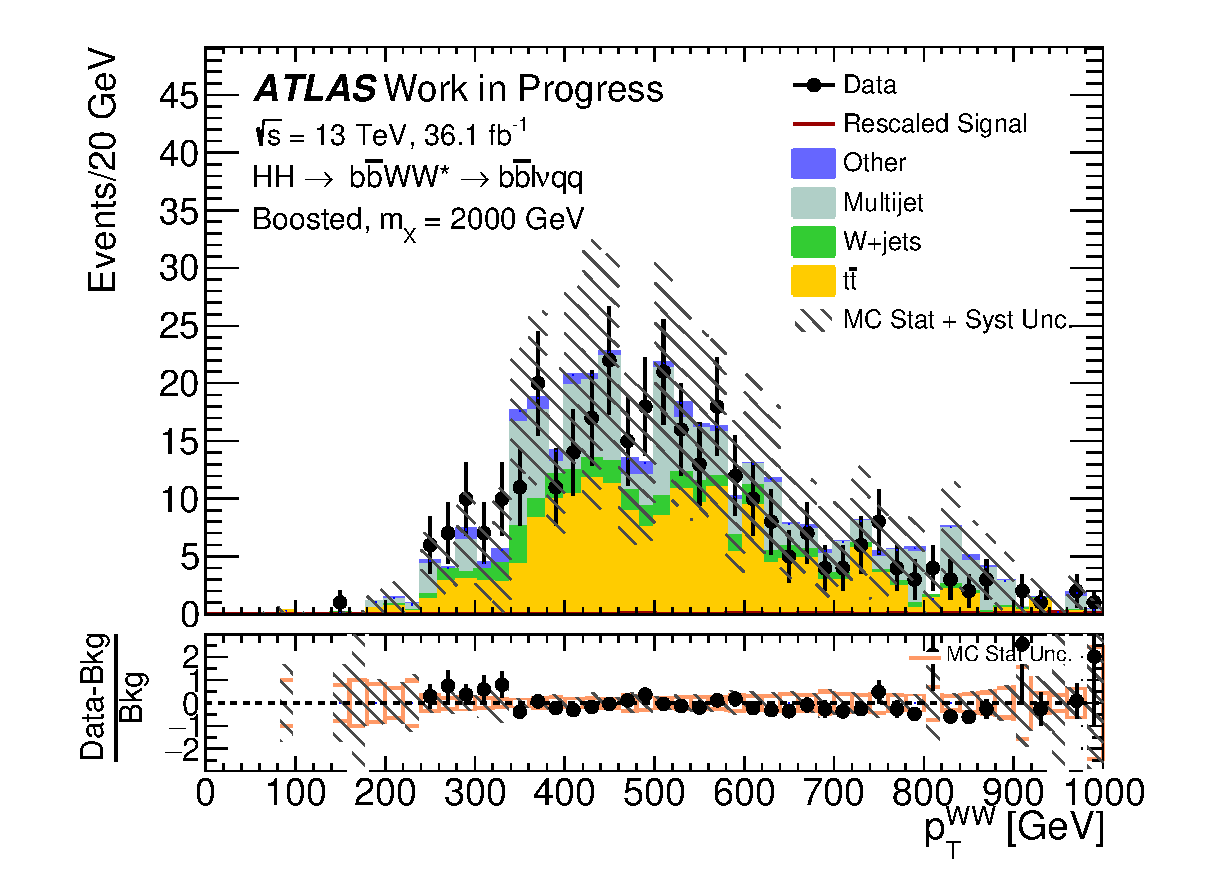
\includegraphics[scale=0.33]{figures/kinplots/C_2tag_mbbcr_elec_presel_met50_WWPt}
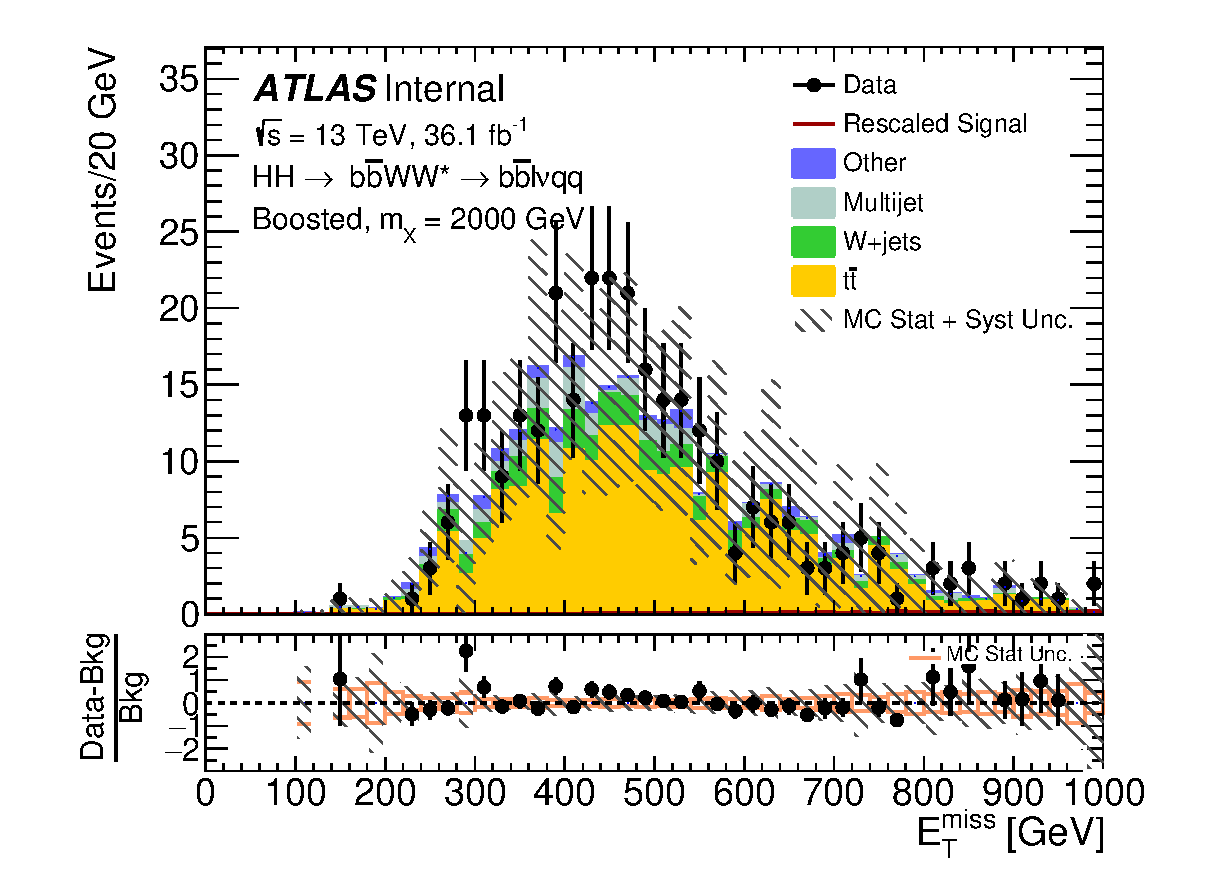
\includegraphics[scale=0.33]{figures/kinplots/C_2tag_mbbcr_muon_presel_met50_WWPt}\\
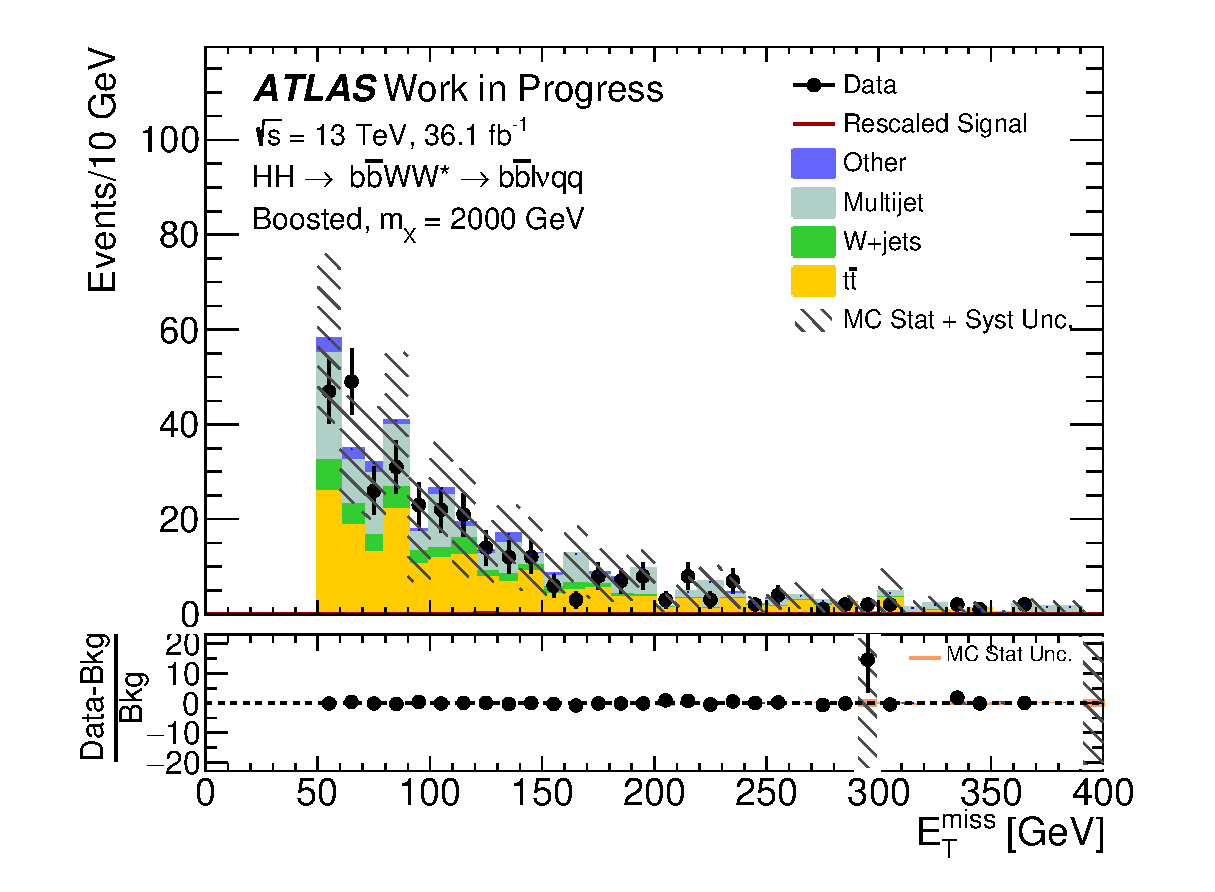
\includegraphics[scale=0.33]{figures/kinplots/C_2tag_mbbcr_elec_presel_met50_MET}
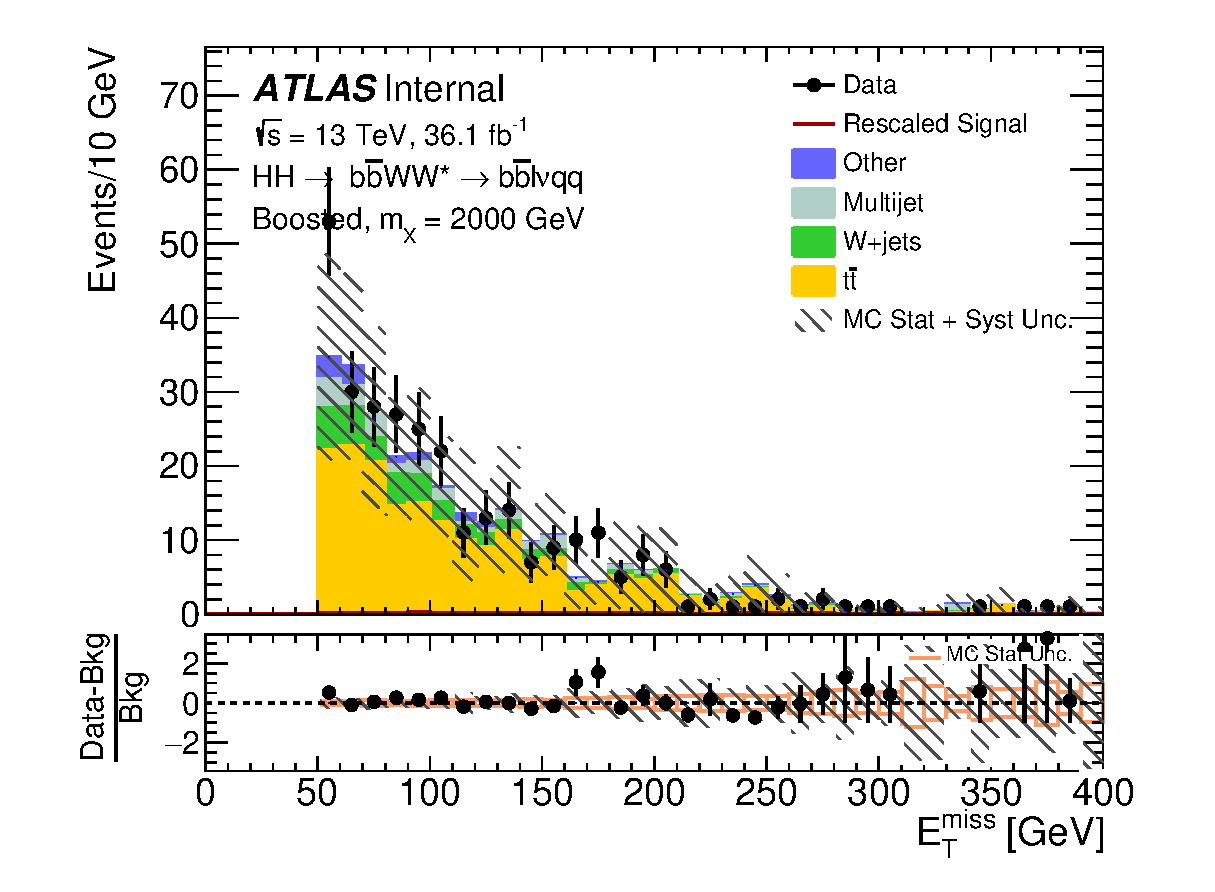
\includegraphics[scale=0.33]{figures/kinplots/C_2tag_mbbcr_muon_presel_met50_MET}\\
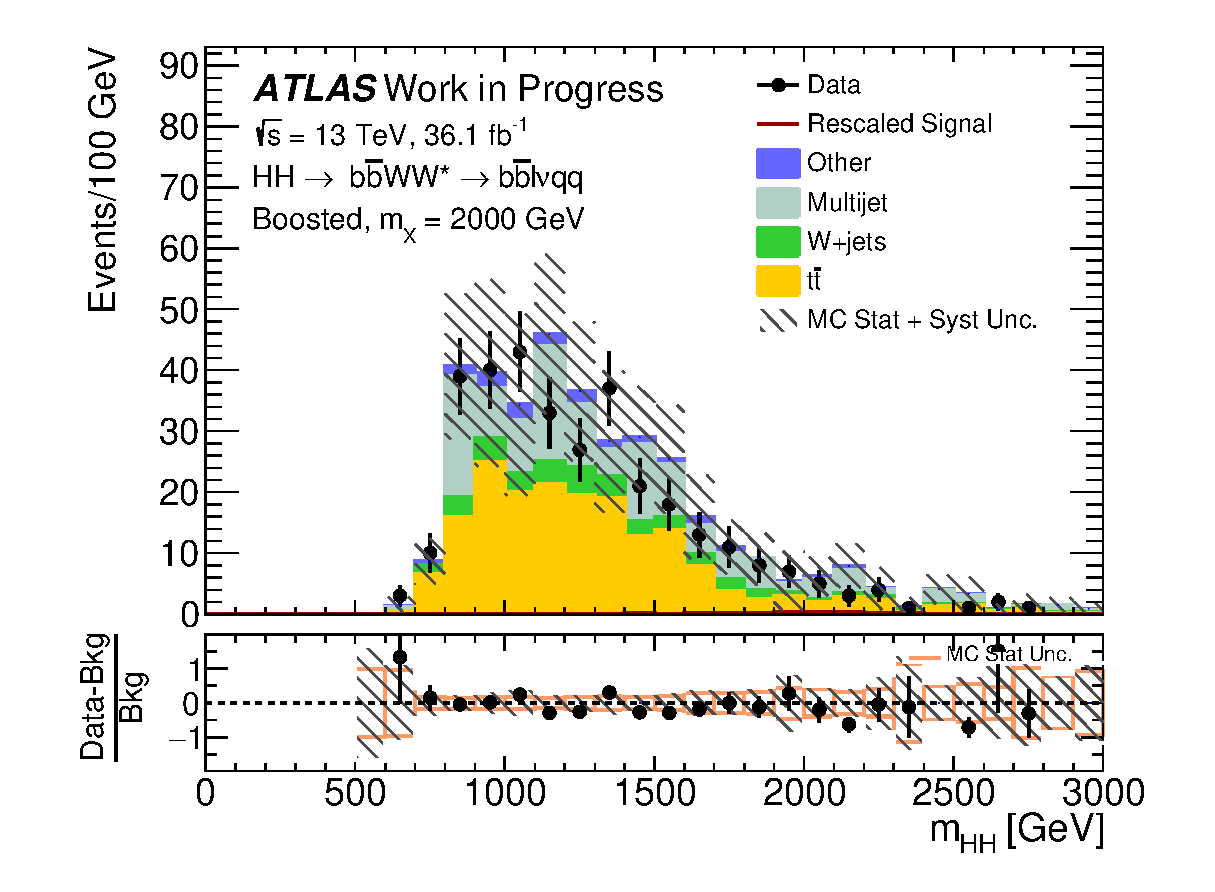
\includegraphics[scale=0.33]{figures/kinplots/C_2tag_mbbcr_elec_presel_met50_hhMassRebin1}
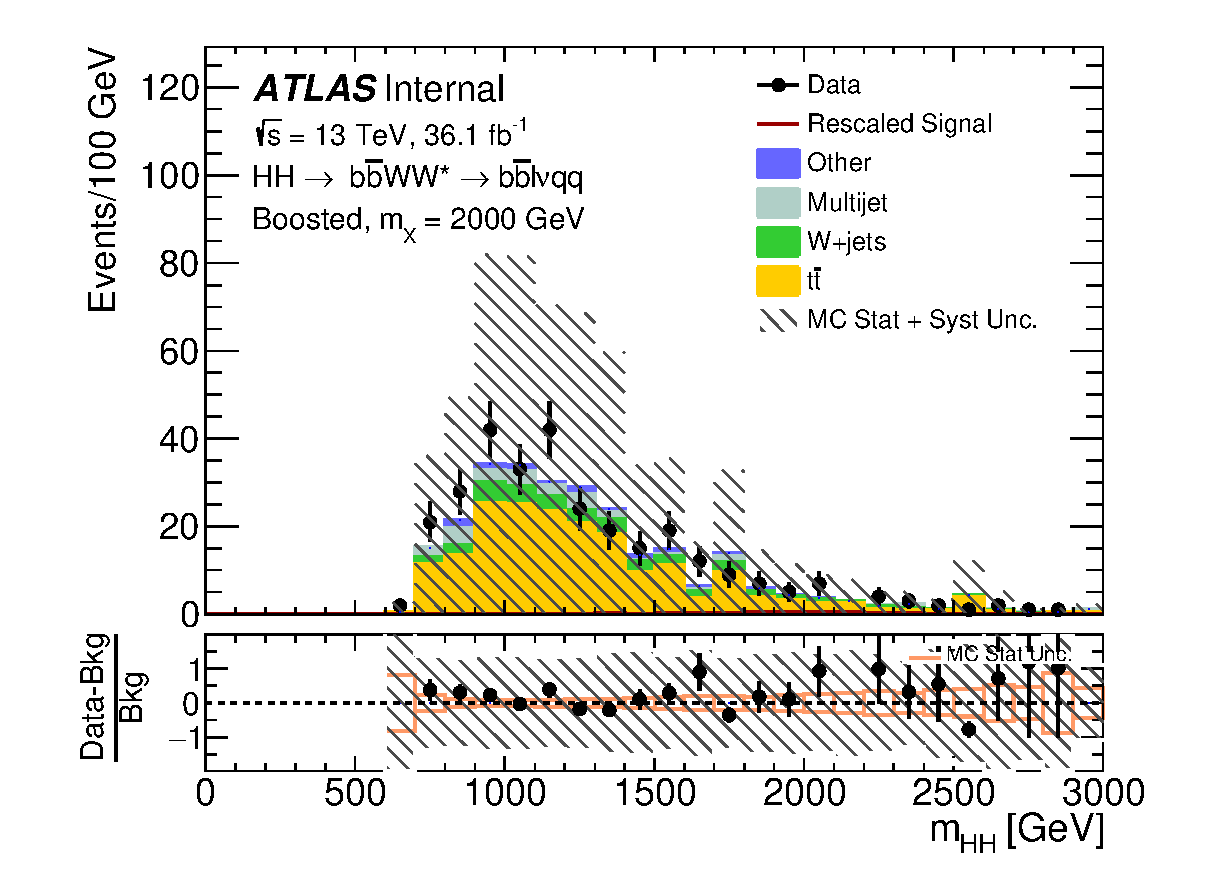
\includegraphics[scale=0.33]{figures/kinplots/C_2tag_mbbcr_muon_presel_met50_hhMassRebin1}
\caption[Kinematic distributions in the mBB control region for the electron and muon channels]{$m_{WW}$, $\pt^WW$, \met, and $m_{HH}$ (from top to bottom) distribution in the mBB control region for the electron (left) and muon (right) channels.}
\label{fig:mbbcr_plots}
\end{center}
\end{figure}
\newpage


\section{Results}

\begin{table}
\small
\begin{center}
\begin{tabular}{c|c|c|c}
$m_X$ [\GeV] & $S$ &  Total Bkg. & Data
\vspace{0.2mm}\\
\hline
2000 & 26.8 $\pm$ 0.5  & 271.0 $\pm$ 10.7  & 268 \\
\end{tabular}
\caption[Data event yields, and signal and background event yields in the final signal region]{Data event yields, and signal and background event yields in the final signal region for the boosted analysis and the scalar $S$ particle hypothesis. The errors shown are the MC statistical uncertainties. For illustration a signal mass point of 2000~\GeV\ is reported in the table. The signal samples are normalized to the expected upper limit cross sections.}  
\label{tab:event_yields_high_new}
\end{center}
\end{table}





The fully-boosted analysis reconstructs the ${m_{HH}}$ distribution and the shape is fit to data using MC signal and background templates. The distribution is fit using 17
bins, with almost uniform width except at low and high $m_{HH}$. %, where the bin width is modified in order to have a MC statistical uncertainty from the MC finite sample-size smaller than 20\%. 
All backgrounds, except multijet, are
simulated using MC generators and normalised using the cross section of the
simulated process. The multijet background is estimated using the ABCD
method, and its normalisation obtained from this method is kept fixed in the fit. The bias due
to possible signal contamination in the ABCD regions was studied
and found to have negligible effect on the result.  The integral of the $m_{HH}$
distribution for the boosted analysis is shown in
Table~\ref{tab:event_yields_high_new}.
\renewcommand{\arraystretch}{1.5}
\begin{table}
\begin{center}
\begin{tabular}{l|c|c|c}
Sample        &  Yield   &  Stats Unc \\  
$t\bar{t}$    &  187.7  & $\pm$ 8.8    \\
W+Jets        &  33.7   & $\pm$ 1.9     \\
QCD           &  34.5   & $\pm$ 5.5     \\
Single-top    &  7.0   & $\pm$ 1.3     \\
Z+Jets        &  4.7    & $\pm$ 0.4        \\
Dibosons      &  3.3    & $\pm$ 0.6      \\
\hline
Prediction    &  271.0  & $\pm$ 10.7       \\
Data          &  268    & - \\
\hline
Data/Pred     &  0.99    & -  \\
\hline
\end{tabular}
\end{center}
\caption[Predicted and observed yields in the mBB control region]{Predicted and observed yields in the mBB control region. Detector modeling
uncertainties, MC background modeling uncertainties and QCD background modeling uncertainties
from ABCD method are considered for the systematic uncertainties.}
\label{tab:boosted_bkgd_mbbcr_yields_new}
\end{table}
\renewcommand{\arraystretch}{1.0}
 
The dominant components of the systematic uncertainties are summarized in Table~\ref{tab:fully_syst}.
\newpage

\begin{table}[p]
\begin{center}
\footnotesize
\begin{tabular}{c|c}
\hline \hline
Uncertainty & Up/Down \\
\hline \hline
SysFT\_EFF\_Eigen\_Light\_0\_AntiKt2PV0TrackJets\_\_1down & -12.9/12.5 \\
SysFT\_EFF\_Eigen\_C\_0\_AntiKt2PV0TrackJets\_\_1down & -12.6/12.1 \\
SysFT\_EFF\_Eigen\_C\_0\_AntiKt2PV0TrackJets\_\_1up & 11.3/-11.9 \\
SysFT\_EFF\_Eigen\_Light\_0\_AntiKt2PV0TrackJets\_\_1up & 11.3/-11.9 \\
SysFATJET\_Medium\_JET\_Comb\_Baseline\_Kin\_\_1up & -6.47/5.95 \\
SysFATJET\_Medium\_JET\_Comb\_Baseline\_Kin\_\_1down & 5.83/-6.43 \\
SysFT\_EFF\_Eigen\_B\_0\_AntiKt2PV0TrackJets\_\_1down & -3.49/2.97 \\
SysFT\_EFF\_Eigen\_B\_1\_AntiKt2PV0TrackJets\_\_1down & -3.32/2.8 \\
SysFT\_EFF\_Eigen\_C\_1\_AntiKt2PV0TrackJets\_\_1down & -2.97/2.45 \\
SysFT\_EFF\_Eigen\_B\_0\_AntiKt2PV0TrackJets\_\_1up & 2.39/-2.94 \\
SysFT\_EFF\_Eigen\_B\_1\_AntiKt2PV0TrackJets\_\_1up & 2.23/-2.78 \\
SysFT\_EFF\_Eigen\_C\_1\_AntiKt2PV0TrackJets\_\_1up & 1.9/-2.45 \\
SysFATJET\_Medium\_JET\_Comb\_Tracking\_Kin\_\_1down & 1.77/-2.38 \\
SysFATJET\_Medium\_JET\_Comb\_Tracking\_Kin\_\_1up & -2.2/1.68 \\
SysFT\_EFF\_extrapolation\_AntiKt2PV0TrackJets\_\_1up & -2.07/1.59 \\
SysFATJET\_JMR\_\_1up & 1.41/-1.97 \\
SysFT\_EFF\_extrapolation\_from\_charm\_AntiKt2PV0TrackJets\_\_1up & -1.62/1.1 \\
SysFT\_EFF\_extrapolation\_AntiKt2PV0TrackJets\_\_1down & 0.963/-1.54 \\
SysPRW\_DATASF\_\_1down & -1.47/0.94 \\
SysJET\_SR1\_JET\_GroupedNP\_1\_\_1down & 0.764/-1.33 \\
SysJET\_SR1\_JET\_GroupedNP\_1\_\_1up & -1.2/0.678 \\
SysFATJET\_JER\_\_1up & 0.574/-1.16 \\
SysFT\_EFF\_Eigen\_Light\_1\_AntiKt2PV0TrackJets\_\_1up & -1.12/0.576 \\
SysFT\_EFF\_extrapolation\_from\_charm\_AntiKt2PV0TrackJets\_\_1down & 0.553/-1.1 \\
SysFATJET\_Medium\_JET\_Comb\_TotalStat\_Kin\_\_1down & -1.03/0.498 \\
\hline 
Total Up & 27.2\\
Total Do & 27.9\\
\hline \hline
\end{tabular}
\caption{List of dominant systematic uncertainties for the fully boosted analysis. The full list of systematic uncertainties is listed in Appendix ~\ref{app:app_fully_syst} }
\label{tab:fully_syst}
\end{center}
\end{table}
\normalsize






\begin{figure}[h]
\begin{center}
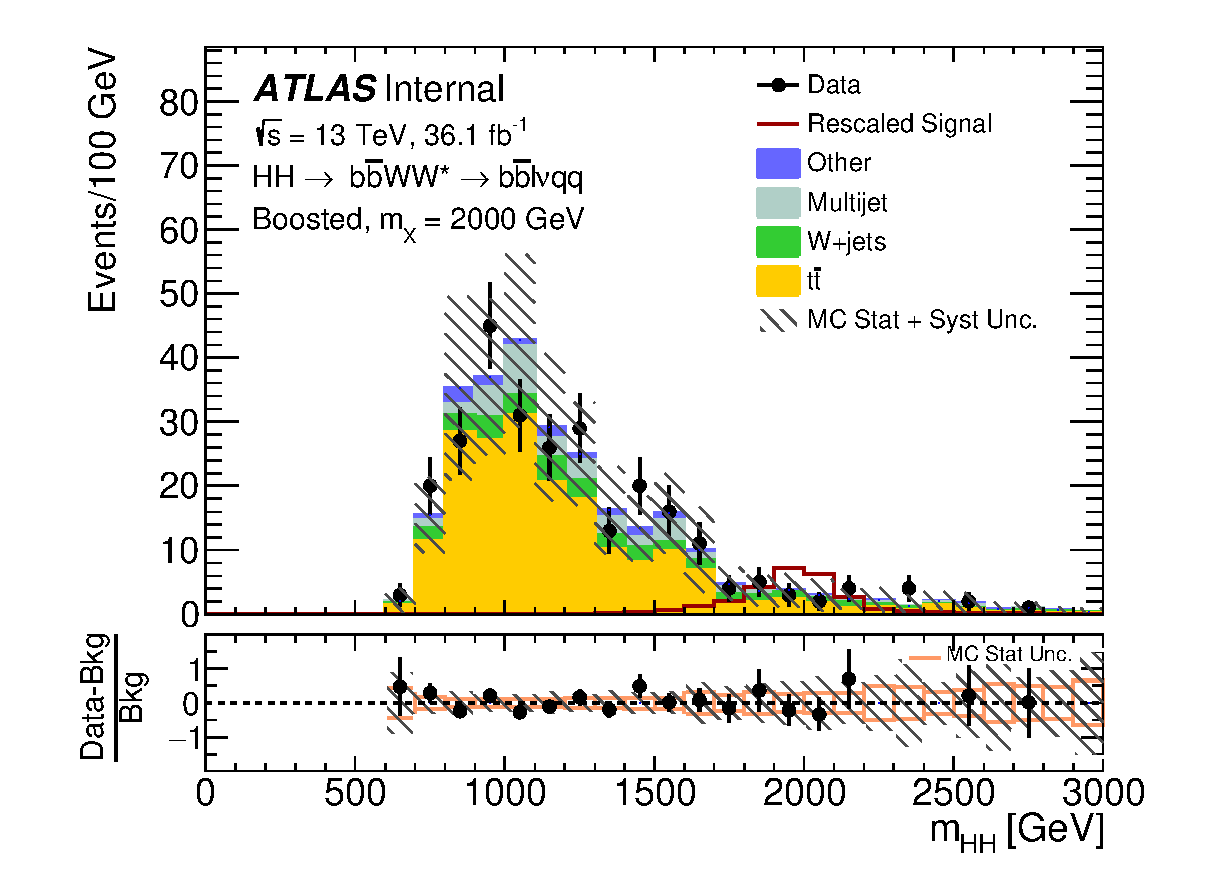
\includegraphics[scale=0.65]{figures/C_2tag_SR_lepton_presel_met50_hhMassRebin1}
\caption{The ${m_{HH}}$ distribution for data and background in the final signal region.}
\label{fig:fully_boost_mhh}
\end{center}
\end{figure}


Figure~\ref{fig:fully_boost_mhh} shows the $m_{HH}$ distribution for
data and the background components for the boosted analysis. Appendix ~\ref{app:sr_john} shows a more complete set of kinematic plots. 
Data are generally in good agreement with the background expectations within the quoted systematic errors.
The signal $m_{HH}$ distribution is shown in the figure for  the scalar resonance.
Figure~\ref{fig:boosted_only_limits_new} shows the observed and the expected
upper limit on the production cross section of the scalar $S$ particle.

\begin{figure}[h]
\begin{center}
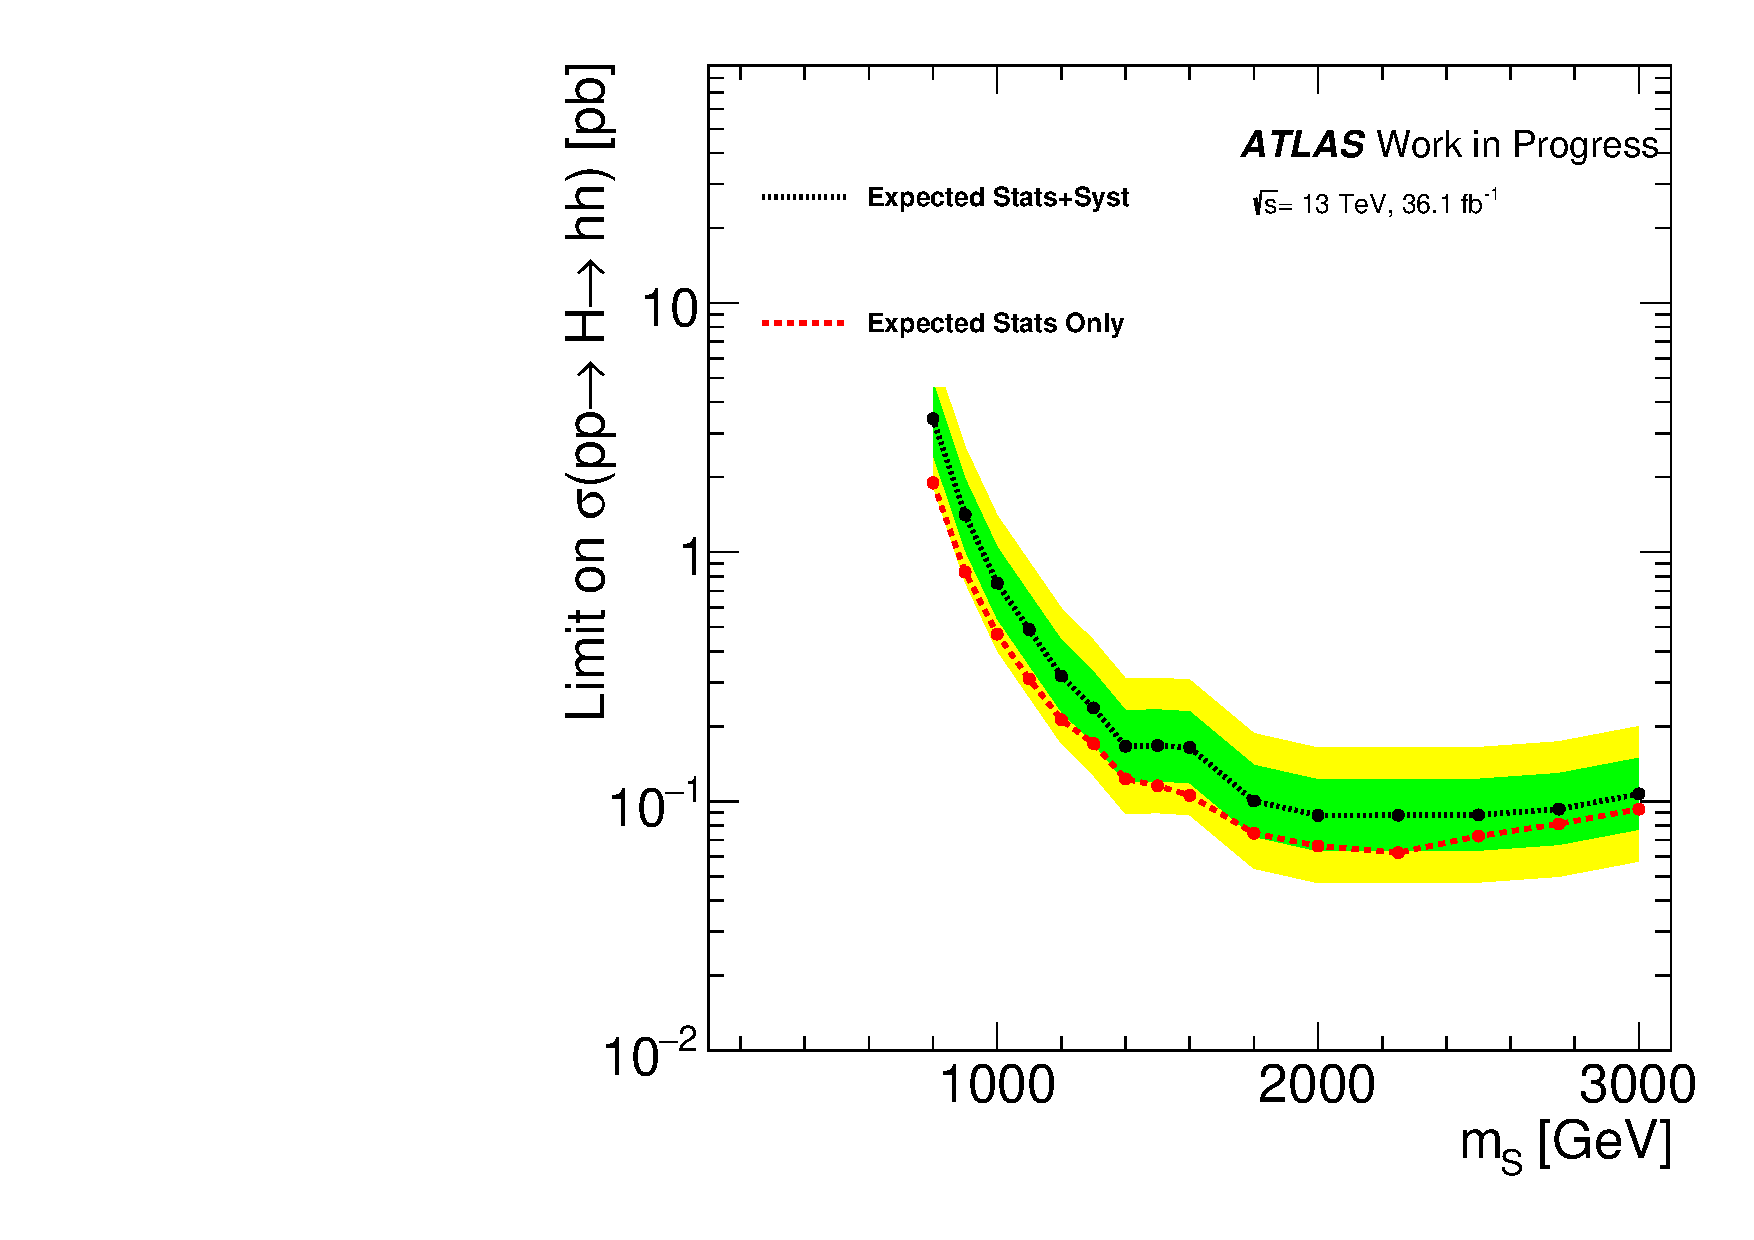
\includegraphics[scale=0.65]{figures/Final_limits}
\caption[Expected and observed upper limits at 95\% CL on the cross section of the resonant pair production for heavy scalar boson S model]{Expected and observed upper limits at 95\% CL on the cross section of the resonant pair production for heavy scalar boson S model. The expected limits without including the systematic errors is also shown to show their impact.}
\label{fig:boosted_only_limits_new}
\end{center}
\end{figure}
\newpage

\section{Conclusion}
The fully-boosted ${HH\rightarrow b\overline{b}WW^{*}}$ semi-leptonic analysis can strengthen the limit on the cross section of the resonant pair production by approximately a factor of 2 over a large range of resonant masses, Figure~\ref{fig:combined_scalar_limit}. \newline
\indent Several improvements can be made to the fully-boosted analysis moving toward the full Run 2 analysis. The isolated lepton trigger that is used for these studies is not suitable for highly collimated topologies and likely leads to a loss of signal efficiency at high resonant masses. A large-R jet trigger would allow for leptons much closer to other objects and could increase the number of events, especially in the high resonant mass region. Additionally, the QCD multijet estimation suffers from a lack of statistics in the C and D regions. This gives a large error on the QCD background estimation. A different method of QCD estimation, such as the matrix method, may be more suitable.\newline
\indent The fully-boosted analysis can be combined with the previous resolved and boosted analysis for the full Run-2 search. By using all three analysis strategies, it is possible to maximize the reach of the analysis across the entire mass range, even extending the range higher. 

